\documentclass[11pt]{article}

\usepackage{deauthor}

\usepackage{upmathgrad2}
\usepackage{UPnotations}

\usepackage{pifont}
\usepackage{amsmath,bm}
\usepackage{amsthm}
\usepackage{bbm}
\usepackage{caption}
\usepackage{amsthm}
\usepackage{pifont}
%\usepackage[ruled,linesnumbered]{algorithm2e}


\newtheorem{definitionnew}{Definition}[section]
\newtheorem{assumption}{Assumption}
\usepackage{wrapfig}
\def\dname{CMLP}
\usepackage{graphicx}
\usepackage{cite}
\usepackage{wrapfig}
\usepackage{tabu}
% \urlstyle{same}
\usepackage{xcolor}
\usepackage{stfloats}
% new package
\usepackage{multirow,fixltx2e}
\usepackage{caption}
\usepackage{float}
\usepackage{microtype}
\usepackage{makecell}
\usepackage{booktabs}


%\newlength\savewidth\newcommand\shline{\noalign{\global\savewidth\arrayrulewidth
%  \global\arrayrulewidth 1pt}\hline\noalign{\global\arrayrulewidth\savewidth}}

\begin{document}
\title{Distilling Causal Metaknowledge from Knowledge Graphs}

% \author{Yuan Meng$^1$, Yancheng Dong$^1$, Shixuan Liu$^2$, Xinzhu Ma$^3$, Chaohao Yuan$^1$, Yue He$^1$, Furui Liu$^4$, Pei Jian$^5$, Peng Cui$^1$}
% \email{{yuanmeng, dongyc20, yuanch22, heyue18 }@mails.tsinghua.edu.cn,
% liushixuan@nudt.edu.cn
% }
% \email{xinzhu.ma@sydney.edu.au, 104256204@qq.com,  jpei@cs.sfu.ca,  cuip@tsinghua.edu.cn}
% \affiliation{$^1$ Tsinghua University $^2$National University of Defense Technology
% \\  $^3$ The University of Sydney  $^4$ Huawei Technologies Ltd.  $^5$ Simon Fraser University}

\author{Yuan Meng, Yancheng Dong, Shixuan Liu, Chaohao Yuan, Yue He, Jian Pei, Peng Cui}% <-this % stops a space
% \email{{yuanmeng, dongyc20, yuanch22, heyue18 }@mails.tsinghua.edu.cn,
% liushixuan@nudt.edu.cn
% }%
% \email{xinzhu.ma@sydney.edu.au, 104256204@qq.com,  jpei@cs.sfu.ca,  cuip@tsinghua.edu.cn}%
% \affiliation{$^1$ Tsinghua University $^2$National University of Defense Technology
% \\  $^3$ The University of Sydney  $^4$ Huawei Technologies Ltd.  $^5$ Simon Fraser University}
% \thanks{Yuan Meng, Yancheng Dong, Chaohao Yuan, Yue He and Peng Cui  are with  Tsinghua University.}% <-this % stops a space
% \thanks{Shixuan Liu is with  National University of Defense Technology.}
% \thanks{Xinzhu Ma is with  the University of Sydney.}
% \thanks{Furui Liu is with  Huawei Technologies Ltd.}
% \thanks{Pei Jian is with Duke University}
% \thanks{J. Doe and J. Doe are with Anonymous University.}% <-this % stops a space
% \thanks{Manuscript received April 19, 2005; revised August 26, 2015.}}



\maketitle

\begin{abstract}
\begin{abstract}
Online crowdsourcing platforms have proliferated over the last few years and cover a number of important domains, these platforms include from worker-task platforms such Amazon Mechanical Turk, worker-for-hire platforms such as TaskRabbit to specialized platforms with specific tasks such as ridesharing like Uber, Lyft, Ola etc.
An increasing proportion of human workforce will be employed by these platforms in the near future.
The crowdsourcing community has done yeoman's work in designing
effective algorithms for various key components, such as incentive design, task assignment and quality control. Given the increasing importance of these crowdsourcing platforms,
it is now time to design mechanisms so that it is easier to evaluate the effectiveness of these platforms. Specifically, we advocate developing benchmarks for crowdsourcing research.

Benchmarks often identify important issues for the community to focus and improve upon.
This has played a key role in the development of research domains as diverse as
databases and deep learning.
We believe that developing appropriate benchmarks for crowdsourcing will ignite further innovations.
However, crowdsourcing -- and future of work, in general -- is a very diverse field
that makes developing benchmarks much more challenging.
Substantial effort is needed that spans across developing benchmarks for
datasets, metrics, algorithms, platforms and so on.
In this article, we initiate some discussion into this important problem and
issue a call-to-arms for the community to work on this important initiative.
\end{abstract}

\end{abstract}


\section{Introduction}
\label{section:introduction}
\section{Introduction}
\label{sec:intro}

Federated Learning (FL) is a distributed machine learning (ML) paradigm that trains a model across a number of participating entities holding local data samples.
% , without exchanging them. 
In this work, we focus on \emph{cross-device} FL that harnesses a large number (up to hundreds of millions) of edge devices with disparate characteristics such as availability, compute, memory, or connectivity
resources~\citep{kairouz2019advances}. %that harnesses potential
% Current applications of FL are designed to scale up to client populations of hundreds of millions or even billions. 
Two challenges to the success of cross-device FL are privacy and scalability. 
FL was originally motivated for improving privacy since data points remain on client devices. 
% and only small model updates were shared to a co-ordinating server.
However, as with other forms of ML, information about training data can be extracted via membership inference or reconstruction attacks on a trained model \citep{carlini2021membership,carlini2020extracting}, or leaked through local updates~\citep{MelisSCS19,geiping2020inverting}. 
Consequently, Secure Aggregation (\SecAgg) protocols were introduced to prevent the server from directly observing individual client updates, which is a major vector for information leakage~\citep{bonavitz2019federated,huba2021papaya}. 
Additional mitigations such as  Differential Privacy (DP) may be required to offer further protection 
against attacks~\citep{dwork2006calibrating,abadi2016deep}, as discussed in Section~\ref{sec:discussion}.
% , as discussed in Section~\ref{sec:discussion}.
%As an additional layer of protection against statistical inference attacks, SecAgg is usually paired with Differential Privacy (DP) \citep{dwork2006calibrating}. To realize the full promise of FL as a privacy-enhancing technology, we need both SecAgg and Differential Privacy.

Ensuring scalability to populations of heterogeneous clients is the second challenge for FL.
% There are many aspects for FL scalability, such as ensuring that model updates can be calculated efficiently 
% by devices with various capabilities and intermittent availability~\citep{bonavitz2019federated}.
% Here, we focus on the communication bottleneck as the primary concern.
Indeed, wall-clock training times are highly correlated with increasing model and batch sizes~\citep{huba2021papaya}, even with recent efforts such as FedBuff~\citep{nguyen2021federated},
% With increasing model and batch sizes, the wall-clock training time increases accordingly~\citep{huba2021papaya}. 
% Despite efforts such as buffered asynchronous aggregation~\cite{nguyen2021federated}, 
and communication overhead between the server and clients dominates model convergence time.
% cross-device FL remains bottlenecked by communication latency between the server and the clients. 
% \karthik{should we mention this paper in a different way? Fedbuff paper doesn't explicitly call out latency as an issue, nor do we run experiments to on async fl ourselves}  \ashkan{I also think the transition can be smoother: first we focus on scalability and billions. Then we say communication is the bottleneck} 
Consequently, compression techniques were used to reduce the communication bandwidth while maintaining model accuracy.
However, a fundamental problem has been largely overlooked in the literature: in their native form, standard compression methods such as scalar quantization and pruning are not compatible with \SecAgg. 
This makes it challenging to ensure both security and communication efficiency.
% at the same time.
% the default method to provide security for client update, 
% presenting an unpleasant dichotomy between security or efficiency. 


% Second, this is the most restricted direction, since upload bandwidth remains more restricted than download. 
% In the US, fixed-line broadband speeds typically achieve a ratio of $3\times$ to $20\times$ more download bandwidth than upload
% bottlenecks remain, and so we seek to reduce the message size of clients by \textit{compression}. 
% Compression has been widely proposed in various ML scenarios, in the form of pruning (removing model parameters) and quantization (reducing fidelity of parameter representation). 
% Indeed, these techniques have been successfully used in FL settings with appreciable improvements in communication while maintaining model accuracy. 
% However, there is a fundamental problem which has been largely overlooked in the literature: in their native form, these compression methods are not compatible with SecAgg, the default method to provide security for client updates. 
% This presents an unpleasant dichotomy: we can have security or efficiency, but not both. 
%
%
% In this paper, we resolve this gap by showing how to modify FL compression techniques to make them security-friendly. We focus on compressing \emph{uplink} updates from clients to the server for two reasons. 
% First, uplink communications are subject to Secure Aggregation protocols to ensure a high security bar, while downlink updates broadcasted by the server are deemed public. 
% Second, upload bandwidth is generally more restricted than download. For instance, according to the most recent FCC report, the ratio of download to upload speeds for DSL/cable providers\footnote{Fixed-line broadband is most relevant since FL is typically restricted to using unmetered connections, usually over Wi-Fi~\citep{huba2021papaya}.} in the US ranges between 3$\times$ to 20$\times$~\citep{fcc-broadband}.
% % This requires some meticulous changes to coordinate clients to use the same global (non-private) hyperparameters, and show that this coordination does not damage model quality. 
% % For the strongest compression methods, we step outside of the SecAgg primitive and propose a new secure primitive, Secure Indexing, which enables the best compression ratios without sacrificing utility. 
% Finally, efficient and secure uplink communication brings several benefits beyond speeding up convergence: 
% lowering communication cost reduces selection bias due to undersampling clients with limited connectivity, improving fairness and inclusivity metrics. 
% It also shrinks the carbon footprint of FL, whose fraction attributable to communication can reach 95\%~\citep{qiu2021first}.
%
%In this paper, w
We address this gap by adapting compression techniques to make them compatible with \SecAgg. We focus on compressing \emph{uplink} updates from clients to the server for three reasons. 
First, uplink communication is more sensitive and so is subject to a high security bar, whereas downlink updates broadcast by the server are deemed public. 
Second, upload bandwidth is generally more restricted than download bandwidth. For instance, according to 
a recent FCC report, 
%the most recent \modif{FCC\footnote{\modif{US Federal Communications Commission.}} report}, 
the ratio of download to upload speeds for DSL and cable providers\footnote{FL is typically restricted to using unmetered connections, usually over Wi-Fi~\citep{huba2021papaya}.} in the US ranges between 3$\times$ to~20$\times$~\citep{fcc-broadband}.
% Fixed-line broadband is most relevant since
% This requires some meticulous changes to coordinate clients to use the same global (non-private) hyperparameters, and show that this coordination does not damage model quality. 
% For the strongest compression methods, we step outside of the SecAgg primitive and propose a new secure primitive, Secure Indexing, which enables the best compression ratios without sacrificing utility. 
Efficient uplink communication brings several benefits beyond speeding up convergence: 
lowering communication cost reduces selection bias due to under-sampling clients with limited connectivity, improving fairness and inclusiveness. 
It shrinks the carbon footprint of FL, the fraction of which attributable to communication can reach 95\%~\citep{qiu2021first}.
In summary, we present the following contributions: 
\begin{itemize}
    \item We highlight the fundamental mismatch between two critical components of the FL stack: \SecAgg protocols and uplink compression mechanisms.
    
    \item We formulate solutions by imposing a linearity constraint on the decompression operator, as illustrated in Figure~\ref{fig:secagg_summary} in the case of TEE-based \SecAgg.
    
    \item We adapt the popular scalar quantization and (random) pruning compression methods for compatibility with the FL stack that require no changes to the \SecAgg protocol.
    
    \item For extreme uplink compression without compromising security, we propose Secure Indexing (\SecInd), a variant of \SecAgg that supports product quantization. %and admits a secure implementation.
\end{itemize}

\begin{figure*}[t]
    \centering
    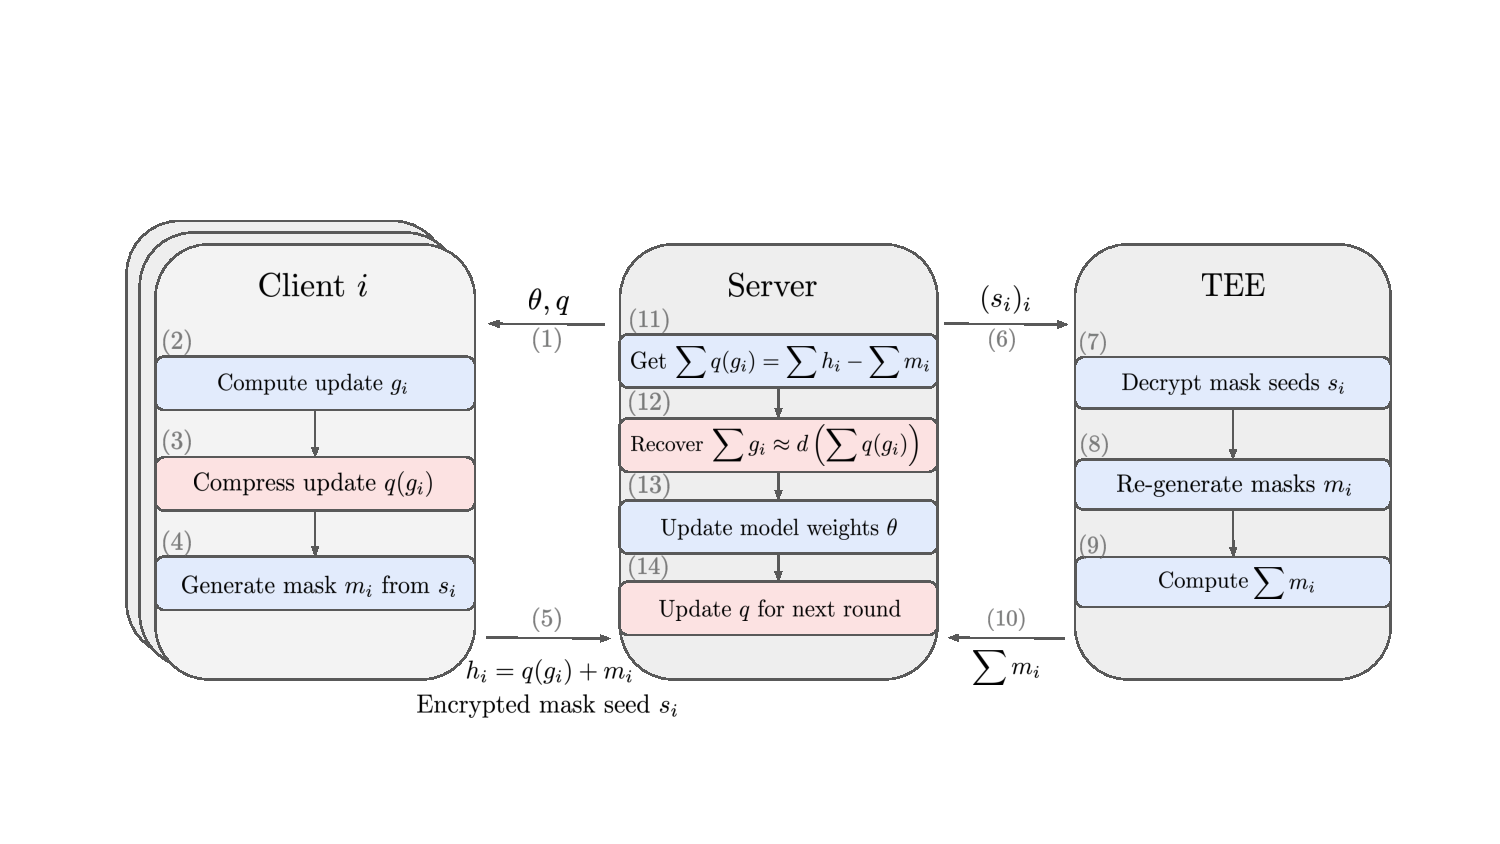
\includegraphics[width=0.8\textwidth]{figs/secagg_summary_new.pdf}
    %\vspace{-5mm}
    \caption{\label{fig:secagg_summary}
    Summary of the proposed approach for one FL round, where we omit the round dependency and \modif{Differential Privacy (DP)} for clarity. Blue boxes denote standard steps and red boxes denote additional steps for uplink compression. Client $i$ computes local model update $g_i$, compresses it with the compression operator $q$, and encrypts it by adding a random mask $m_i$ in the compressed domain, hence reducing the uplink bandwidth (steps 2--4). The server recovers the aggregate in the compressed domain by leveraging any \SecAgg protocol \modif{(steps 7--13, with a TEE-based \SecAgg, see Section~\ref{subsec:secagg})}. Since the decompression operator $d$ is linear, the server can convert the aggregate back to the non-compressed domain, up to compression error (step 12). As with the model weights $\theta$, the compression operator $q$ are also periodically updated and broadcast by the server (step 14). 
    In Section~\ref{sec:method}, we apply the proposed method to scalar quantization and pruning without impacting \SecAgg and propose Secure Indexing, a variant of \SecAgg for extreme uplink compression with product quantization. See Section~\ref{subsec:secagg} for details about \SecAgg and Section~\ref{sec:discussion} for a discussion on~DP.
    }
    \vspace{-3mm}
\end{figure*}



% Our focus in this paper is on 

%Second, scaling cross-device (synchronous) FL to millions of clients with various capabilities and intermittent availability \citep{bonavitz2019federated} suffers from diminishing returns: the wall-clock training time plateaus as the number of clients keeps increasing~\citep{huba2021papaya}. Even though this challenge can be addressed by leveraging the buffered asynchronous aggregation technique proposed by \cite{nguyen2021federated}, compatible with DP and SecAgg, the asynchronous protocol remains bottlenecked by communication latency between the server and the clients.


%Considering the above privacy and scalability goals, we focus on enabling efficient FL communications while keeping a high privacy bar. In addition to the primary objective of speeding up convergence, reducing communication costs brings other significant benefits. Lowering communication requirements addresses selection bias due to undersampling clients with limited connectivity, improving fairness and inclusivity metrics. Better communication efficiency shrinks the carbon footprint of FL, whose fraction attributable to communication can reach 95\%~\citep{qiu2021first}. %Finally, training larger model in FL would be a possibility, when the communication cost is reduced, because local memory or compute requirements can be addressed by modifying the local training loop, for instance with gradient checkpointing \citep{chen2016training}. However, some form of compression would be required to enable efficient communication.


%First, compressing model updates from the client to the server presents several challenges due to compatibility with SecAgg and is an area suitable for further research. 
%Second, upload bandwidth is generally more restricted than download. For instance, according to the most recent FCC report, the ratio of download to upload speeds for DSL/cable providers in the US ranges between 3$\times$ to 20$\times$~\citep{fcc-broadband}. We consider broadband speeds here because devices participate in the FL training while connected to fixed broadband, usually through Wi-Fi~\citep{huba2021papaya}.




% Hence, FL provides the ability to leverage data from massive client populations while ensuring the security and privacy of the client data.
% Go further: compatibility with DP / compression as a mitigation techniques of attacks
% Model and gradient compression intrinsically different.
%  Why not having the secure enclave perform the aggregation?






\section{Preliminaries and Problem Statement}
\label{section:model}
\subsection{Definitions and Notations}

In this paper, we follow the definition of knowledge graph as in~\cite{ji2021survey}:
\begin{definitionnew}
A \textbf{Knowledge Graph (KG)} is defined as $\mathcal{G}=(\mathcal{E},\mathcal{R},\mathcal{F})$, where
$\mathcal{E}$, $\mathcal{R}$ and $\mathcal{F}$ are sets of entities, relations and facts, respectively.
Every fact is a triple $(e_h,R,e_t) \in \mathcal{F}$, where $e_h, e_t\in \mathcal{E}$ and $R \in \mathcal{R}$ are head entity, tail entity and the relation between entities, respectively. Without loss of generality, we simultaneously represent a fact as $R(e_h,e_t)$.
\end{definitionnew}

%Here we introduce a similar data structure with KG: heterogeneous information graph, following the definition in ~\cite{sun2011pathsim}:

%\begin{definition}
%A \textbf{heterogeneous information network (HIN)} \cite{sun2011pathsim}is a directed graph $G=(V, E, \Phi, \Psi)$, where $V$ is the set of nodes (or entities) of the graph; $E \subseteq V \times V$ is the set of edges connecting the nodes in $V$; and $\Phi$ and $\Psi$ are functions for labeling nodes and edges. We have $\Phi: V \rightarrow \mathcal{A}$, where $\mathcal{A}$ is the set of node classes, and $\Psi: E \rightarrow \mathcal{B}$, where $\mathcal{B}$ is the set of edge types.
%\end{definition}

%Given a complex heterogeneous information network, it is necessary to provide its meta level (i.e., schema-level), which is called network schema.

%\begin{definition}
%A \textbf{network schema}\cite{sun2011pathsim} is a meta template for a HIN $G=(V, E)$ with the object type mapping $\phi: V \rightarrow \mathcal{A}$ and the link mapping $\psi: E \rightarrow \mathcal{R}$, which is a directed graph defined over object types $\mathcal{A}$, with edges as relations from $\mathcal{R}$, denoted as $T_G=(\mathcal{A}, \mathcal{R})$.
%\end{definition}

%Generally, both KG and HIN are graph-based models for representing relational data.
%The HIN provides this constraint via labeling function $\Phi$, requiring each node to correspond to a single node type, whereas the description of node types is not necessary for the general KG.
%The relationship between KG and HIN is a subject of debate in academia.
%A recently published article by


%\begin{definition}
%A \textbf{meta-path}\cite{sun2011pathsim} $\mathcal{P}$ is a path defined on the graph of network schema $T_G=(\mathcal{A}, \mathcal{R})$, and is denoted in the form of $A_1 \stackrel{R_1}{\longrightarrow} A_2 \stackrel{R_2}{\longrightarrow} \ldots \stackrel{R_l}{\longrightarrow} A_{l+1}$, which defines a composite relation $R=R_1 \circ R_2 \circ \ldots \circ R_l$ between type $A_1$ and $A_{l+1}$, where - denotes the composition operator on relations.
%\end{definition}




%A Knowledge graph(KG) $\mathcal{G}=(\mathcal{E},\mathcal{R},\mathcal{T})$ can be regarded as a kind of heterogeneous information network\lsx{?}, where
%$\mathcal{E}$
% $\mathcal{E} = \{e_1,e_2,\cdots,e_{|\mathcal{E}|}\}$
%is the \textit{entity} set,
% of $\mathcal{G}$
% and $|\mathcal{E}|$ is the number of the entities in $\mathcal{G}$;
%$\mathcal{R}$
% $\mathcal{R} = \{R_1,R_2,\cdots,R_{|\mathcal{R}|}\}$
%is the \textit{relation} set,
% in $\mathcal{G}$, which includes $|\mathcal{R}|$ different types of relations;
%and $\mathcal{T} \in \mathcal{E} \times \mathcal{R} \times \mathcal{E}$ is the \textit{fact} set, where the facts are represented as triples.
%A triple can be denoted as $<e_h,R,e_t>$ or $R(e_h,e_t)$,
%where $e_h$ is the head entity, $e_t$ is the tail entity, and these two entities are connected by the relation $R$ to form a \textit{fact} in $\mathcal{G}$.
% Under the closed world assumption (CWA)
% ~\cite{hogan2021knowledge}, the fact set includes all the existing relationships between any entity pair from $\mathcal{R} \times \mathcal{R}$.
First-order logic (FOL) offers a pivotal way to represent real-world knowledge for reasoning. Horn rules, as a special and typical case of FOL rules, propose to represent a target relation by a body of conjunctive relations.

\begin{definitionnew}
\label{def:horn_rule}
A \textbf{Horn Rule}, generally chain-like, is given as,
\begin{equation*}
    R_h(x,y) \leftarrow R_{b_1}(x,z_1) \circ \cdots \circ R_{b_l}(z_{l-1},y)
\end{equation*}
where, $R_h(x,y)$ signifies the rule head (target relation) that we wishes to reason and $R_{b_1}(x,z_1) \circ \cdots \circ R_{b_l}(z_{l-1},y)$ is the rule body (relation path). For simplicity, we denote a Horn rule as $R_h:\mathbf{R_b}$, where $\mathbf{R_b}=[R_{b_1}, \cdots, R_{b_l}]$. To reason $R_h$, the size of the rule space is $|\mathcal{B}_h|$.
Every \textbf{closed path} of such Horn rule is required to: 1) connect $(x,y)$ via the rule body, which is a sequence of relations $\mathbf{R_b}$, and 2) ensure $(x,y)$ are accessible directly via the target relation $R_h$. Closed paths are also known as \textbf{rule instances}.
\end{definitionnew}

%Each KG corresponds to a concept set $\mathcal{C}$, and each concept $C \in \mathcal{C}$ corresponds to a concept-specific entity set  $\mathcal{E}_C \in \mathcal{E}$.
%Therefore the concept can be treated as the label of the entity class.


\subsection{Problem Statement}
The goal of this work is to learn the \textbf{causal rule} that is formalized as the horn rule.
Specifically, the objective of traditional logical rule learning is to assign a plausibility score $\mathbf{S}(R_h|\mathbf{R_b})$ to each rule in the discovered rule space, which can be subsequently aggregated to answer queries about the KG.
Currently, plausibility scores are defined over closed paths (e.g., the PCA confidence for AMIE~\cite{galarraga_amie_2013}), which are correlational observations.
We have demonstrated that these scores are prone to spurious correlations and therefore result in inaccurate predictions under OoD settings, in Sec. \ref{section:introduction}.
Therefore the other aim is to give a plausibility score based on causal strength.


In this paper, the causal rules are mined for link prediction in KG.
We follow the commonly accepted problem definition of link prediction in KG~\cite{rossi2021knowledge,tiwari2021revisiting}:
given an observed KG $\mathcal{G}$ with missing facts, our goal is to predict the correct entity for an given query $(e_h,R_h,?)$ (or $(?,R_h,e_t)$).
%For simplicity, we refer to the known entity in the prediction as source entity and the entity to be predicted as target entity.
% Specifically, the objective of logical rule learning is to assign a plausibility score $\mathbf{S}(R_h|\mathbf{R_b})$ to each rule in the discovered rule space, which are subsequently aggregated to rank all possible answers. Currently, plausibility score are defined over closed paths (e.g., the PCA confidence for AMIE~\cite{galarraga_amie_2013}), which are associational observations. We elaborate these scores are prone to spurious correlations and therefore result in inaccurate predictions under OoD settings, in Sec. \ref{section:model}. 


% introduce the representation
% \section{Structural Causal Knowledge Model}

\section{Proposed Method: ~\dname}
\label{section:model}
In this section, we introduce the proposed approach~\dname~ which learns causal rules for KG link prediction.
\dname~ first transforms the relational data into the propositional data to conduct statistical analysis (Sec. \ref{sec:tabularnizar}).
Then \dname~ presents a local causality identification algorithm based on the $d$-seperation criterion to efficiently mines interpretable causal rules (Sec. \ref{sec:discovery}).
Finally, a specific causation-based score is applied in predictor to answer the queries with learned causal rules (Sec. \ref{sec:link_pred}).
The pipeline of \dname~is illustrated in Fig. \ref{fig:framwork}.
% the proposed CFLP first transforms the input data from graph representation into tabular representation for better  (Sec. \ref{sec:tabularnizar}). Then we design a local causality identification algorithm based on the $d$-seperation criterion to efficiently mines interpretable causal rules (Sec. \ref{sec:discovery}).
% Finally, a specific link prediction approach is applied to integrates the weight information  derived from the causality test (Sec. \ref{sec:link_pred}).
\begin{figure*}[htbp]
\begin{center}
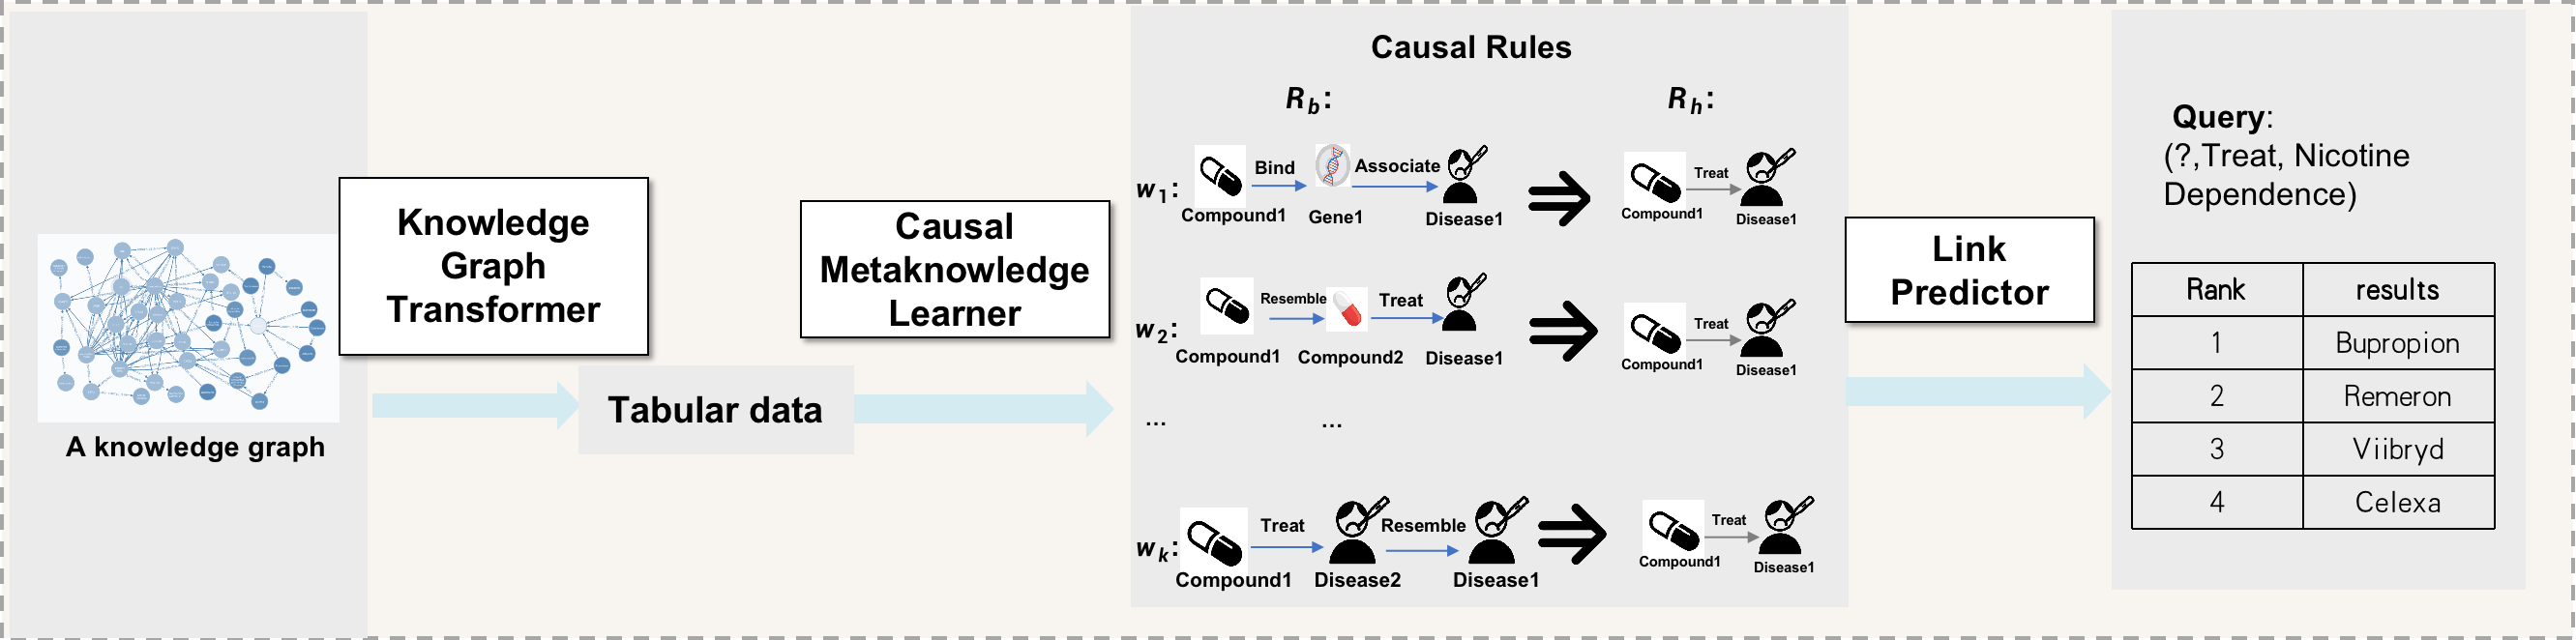
\includegraphics[width=18cm]{submissions/causal-meta-knowledge/figures/cmlp.png}
\end{center}
\caption{The framework of~\dname. Particularly, CFLP first transforms the relational data into propositional data for better statistical analysis. Then it mines interpretable causal rules, which can be interpreted as a kind of metaknowlege\cite{evans2011metaknowledge}.
Finally, a plausibiliy score derived from the causality test is applied in predictor to rank the answers of the given query.}
\label{fig:framwork}
\end{figure*}
\begin{figure*}[hbp]
\begin{center}
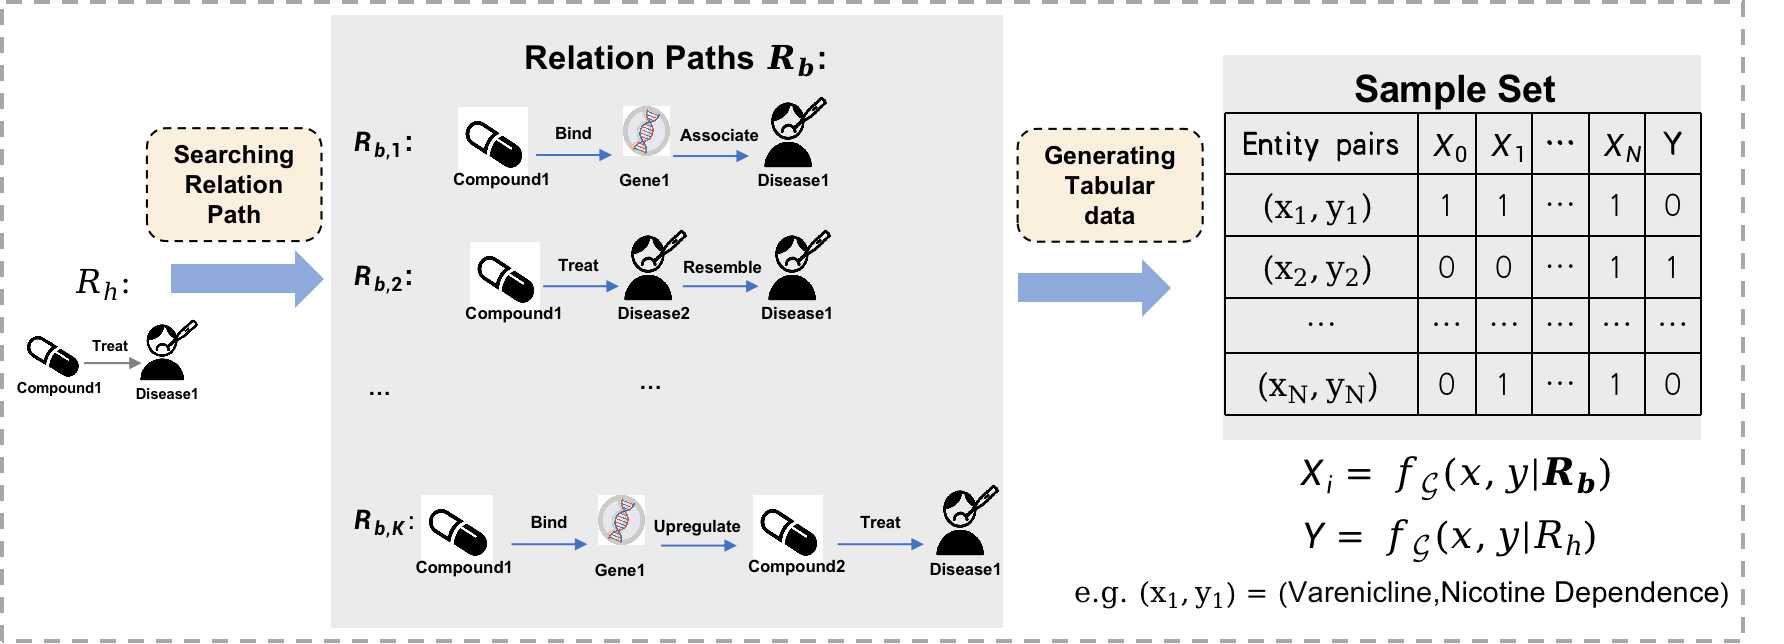
\includegraphics[width=14cm]{submissions/causal-meta-knowledge/figures/transformer.jpg}
\end{center}
\caption{The process of knowledge graph transformer}
\label{fig:tabular}
\vspace{-0.6cm}
\end{figure*}

\subsection{Knowledge Graph Transformer}
\label{sec:tabularnizar}
% The inference rules are generally defined at the concept level, and the link prediction tasks are operated at the entity level.
% For example, based on the inference rule of relation \texttt{Treats(Compound, Disease)}, we can conduct a specific query $(?, Treat, Nicotine Dependence)$.
% In~\dname, to learn the conceptual causal rules, we first introduce the possible causes of a conceptual fact.
Traditional causal discovery algorithms are defined on propositional data, with well-defined variables and samples, which do not exist in relational data like KGs.
Therefore, we give the definition and scope of the variables we study in the causal discovery phase by mapping the potential causes and queried relations into variables.
Then we give the practical approach for transforming KG into tabular data, whose horizontal axis are the variables we defined.
The process is shown schematically in Fig.~\ref{fig:tabular}



\subsubsection{Causal variables in KG}
The causal rule can be interpreted as a description of causal relationship between the body and the head.
Naturally, we formulate variables based on the elements of rules.
% Due to the difficulty of data acquisition, for knowledge graphs extracted from texts, there is often no corresponding attribute information of entities corresponding to them.
% The connection information between a pair of entities is the only source we can access to infer the missing link between them.
% For example, the genetic connection structure is
%$Compound \stackrel{Bind}{\longrightarrow} Gene \stackrel{Associate}{\longrightarrow} Disease$.
% $Bind(Compound, Gene) \circ Associate(Gene, Disease)$.

% \yym{a sample to explain this model}
% \yym{rewrite}
% Relational causal model (RCM) is a Baysian network, which encodes the causal dependency for the relational data.
% RCM is designed for the relational database, in which the entity classes and relations are represented as tables with attributes.
% RCM depends on the known relational skeleton, which includes all the relations between entities, to infer the unknown attributes.
% However, in practice, the relations among entities are missing and are treated as learned target in some application, such as link prediction task for KG.
% And normally, the attributes of entity classes are lack in the real KG.
% Therefore in this section, we will build a causal model for the relations in KG without information of the entities' attributes.
% With the relational skeleton, RCM can represents the conditional independent relationship among the attributes of the entity class.

% We first introduce several concepts and definitions, which are the components of our model.

\noindent
% \begin{definition}
% \textbf{Knowledge Graph Schema(KGS.)}
% A KGS $S=(\mathcal{C}^S, \mathcal{R}^S, \mathcal{V},\mathcal{B} )$ is a directed graph, defined on a KG $\mathcal{G}=(\mathcal{E},\mathcal{R},\mathcal{T})$ with relation set $\mathcal{R}^S \in \mathcal{R}$,
% where each vertice $v \in \mathcal{V}$ corresponds to a concept $C \in \mathcal{C}^S$ and each edge $b \in \mathcal{B}$ corresponds to a relation $R  \in \mathcal{R}^S$.
% \end{definition}

%\begin{definition}
%A \textbf{meta structure} connecting source node $n_h$ and target node $n_t$
%$M=(\mathcal{C}_M, \mathcal{R}_M, \mathcal{V},\mathcal{B}, n_h, n_t)$ is a directed graph, defined on a KG $\mathcal{G}=(\mathcal{E},\mathcal{R},\mathcal{T})$ with concept set $\mathcal{C}$, where $\mathcal{V}$ and $\mathcal{B}$ are node set and edge set, respectively, and each node $v \in \mathcal{V}$ corresponds to a concept $C \in \mathcal{C}_M$ each edge $b \in \mathcal{B}$ corresponds to a relation $R  \in \mathcal{R}_M$.

% with relation set $\mathcal{R}_M \in \mathcal{R}$,
% where each vertice $v \in \mathcal{V}$ corresponds to a concept $C \in \mathcal{C}^S$ and each edge $b \in \mathcal{B}$ corresponds to a relation $R  \in \mathcal{R}^S$.
%\end{definition}
% A relation path is a template and proxy of sub-KG that describes a kind of topological relationship between a pair of concepts.
% Therefore, the bodies of rules can be conceived as topology attributes for all concept pairs.
% And the head of the rule is also a special attribute.
% Here we give the some officially definitions to introduce the assumption on the causes of concept-level links in KG.
%The conceptual triple is a kind of meta structure.
%There is a slightly difference with the past definition of meta structure \cite{huang2016meta}: we do not restrict the meta structure to be a directed acyclic graph (DAG), because the direction of the connection from head entity to tail entity may not be unidirectional or directed under different relational semantics, such as $<Compound,Associate,Disease>$\lsx{?}

%\begin{definition}
%A \textbf{Rule-induced Variable} $X=(C_h,C_t).M$ is defined on two concepts $C_h$ and $C_t$ and a meta structure $M$, where $C_h$ and $C_t$ correspond to $n_s$ and $n_t$ in $M$, respectively.
%\end{definition}

\begin{definitionnew}
For entity pair $(x,y)$, its \textbf{Rule-induced Variable} $X_k=f_{\mathcal{G}}(x,y|\mathbf{R_b}^k)$, where $\mathbf{R_b}^k$ corresponds to the rule body in the $k$-th rule $R_h:\mathbf{R_b}^k (k \in \{1, ..., |\mathcal{B}_h|\})$. The assignment function $f_{\mathcal{G}}(\cdot|\mathbf{R_b})$ can be either connectivity feature or path count for $\mathbf{R_b}$ in KG $\mathcal{G}$.
\end{definitionnew}

The head of rule also induces a special variable $Y=f_{\mathcal{G}}(x,y|R_h)$.
In the real link prediction task, the queries are normally on a specific relation, such as \texttt{Treat} in drug repurposing.
Therefore, the causal rule mining problem is to discovery the causal relationship between variables $X_k=f_{\mathcal{G}}(x,y|\mathbf{R_b}^k), k \in \{1, ..., |\mathcal{B}_h|\}$ and variable  $Y=f_{\mathcal{G}}(x,y|R_h)$.
% With the definition of variables, the causal rule discovery is transformed to the traditional causal discovery task
Then we introduce the practical approach that we transform the KG into tabular data for causality analysis.

% In this paper, we treat the \textit{entity pair} as the study unit, since we focus on the generation mechanism of the relations in KG without the attributes of a single entity and each relation must involve two entities.
% The concept pair label the classes of the entity pair, and the meta structure $M$ reflect the connection characteristics between the two entities. Besides, We assume the concept-level connection information of given concept pair as the factors, which potentially \textit{cause} the specific relation between these two concepts.

%\begin{assumption}
%\textbf{Candidate causes of conceptual triples:}
%\label{ass:candidata}
%given a variable $(C_h,C_t).M_q$ defined by a queried conceptual triple $M_q=<C_h,R,C_t>$, the candidate causes of it are any variables $(C_h^c,C_t^c).M_c$ defined by the meta structure $M_c=(\mathcal{C}_M, \mathcal{R}_M, \mathcal{V},\mathcal{B}, n_h, n_t)$, where $C_h^c=C_h$ and $C_h^t=C_t$.
% and $C_1^{Ca} \cap C_1 \neq \emptyset, C_2^{Ca} \cap C_2 \neq \emptyset$.
%\end{assumption}

% \begin{assumption}
% \textbf{Candidate causes of rule-induced variables:}
% \label{ass:candidata}
% given a variable $X_k=f_{\mathcal{G}}(x,y|\mathbf{R_b}^k)$ defined by the $k$-th rule to reason queried relation $R_th$, the candidate causes of it are any variables $X_j=f_{\mathcal{G}}(x,y|\mathbf{R_b}^j)$ defined by other rule $j(j\neq k)$ in the rule space.
% % and $C_1^{Ca} \cap C_1 \neq \emptyset, C_2^{Ca} \cap C_2 \neq \emptyset$.
% \end{assumption}

% A KGS-based variable $X=f(\mathcal{G},S,e^h,e^t)$ is a function of two entity variables $e^h,e^t$, with each entity variable corresponding to two nodes of KGS $S=(\mathcal{C}^S, \mathcal{R}^S, \mathcal{V},\mathcal{B} )$, where the KGS is defined on KG $\mathcal{G}$.


% \begin{itemize}
%     \item a set of meta structural attributes$(C_h,C_t).\mathcal{M}$
%     \item a set of parents $\text{Pa}((C_h,C_t).M)=\{(U_1,\dots,U_l\}$, where each $U_i$ has the form $C_h,C_t).M_i$;
%     \item a conditional probability distribution (CPD) that represents $P(C_h,C_t).M| C_h,C_t).M)$
% \end{itemize}
% A KGS-based dependency model $\mathcal{M}_\theta$ has two parts:

% 1. The structure $\mathcal{M}=(\mathcal{V},\mathcal{D})$: a directed graph with each node corresponding to a KGS-based variables $X \in \mathcal{V}$ and each edge corresponding to a schema-level dependency defined between two variables in $V$.

% 2. The parameters $\theta$: a conditional probability distribution
% \begin{equation}
% \begin{aligned}
% P(X=f(\mathcal{G},S^X,e^h,e^t)|\text{~parents}(X))
% \end{aligned}
% \end{equation}
% for each KGS-based variable with the entity variables and $\text{parents}(X)=\{Y|Y=f(\mathcal{G},S^Y,e^h,e^t)\}$ is the set of parent KGS-based variables, which have the same entity variable pair with $X$.




% Given the entity set, if we can model the





% \noindent
% \begin{definition}
% \textbf{KGS-based variable}
% A KGS-based variable $X=f(\mathcal{G},S,e^h,e^t)$ is a function of two entity variables $e^h,e^t$, with each entity variable corresponding to two nodes of KGS $S=(\mathcal{C}^S, \mathcal{R}^S, \mathcal{V},\mathcal{B} )$, where the KGS is defined on KG $\mathcal{G}$.
% \end{definition}

% The mapping function $f$ is as following:
% $$
% f(\mathcal{G},S,E^h,E^t)=\left\{
% \begin{aligned}
%     1  & \text{~~if there is an instance path of KGS~}
%        S \text{~with~} e^h,e^t \text{in} \ \mathcal{G}.\\
%     0 & \text{~~otherwise}.
% \end{aligned}
% \right.
% $$


% \begin{definition}
% \textbf{Schema-level dependency}
% A schema-level dependency $Y \to X$, defined between two KGS-based variables $X=f(\mathcal{G},S^X,e^h,e^t)$ and $Y=f(\mathcal{G},S^Y,e^h,e^t)$, is a directed probabilistic dependence from  $Y$ to $X$, which have the same entity variables.
% \end{definition}

% \begin{definition}
% \textbf{KGS-based dependency model}
% A KGS-based dependency model $\mathcal{M}_\theta$ has two parts:

% 1. The structure $\mathcal{M}=(\mathcal{V},\mathcal{D})$: a directed graph with each node corresponding to a KGS-based variables $X \in \mathcal{V}$ and each edge corresponding to a schema-level dependency defined between two variables in $V$.

% 2. The parameters $\theta$: a conditional probability distribution
% \begin{equation}
% \begin{aligned}
% P(X=f(\mathcal{G},S^X,e^h,e^t)|\text{~parents}(X))
% \end{aligned}
% \end{equation}
% for each KGS-based variable with the entity variables and $\text{parents}(X)=\{Y|Y=f(\mathcal{G},S^Y,e^h,e^t)\}$ is the set of parent KGS-based variables, which have the same entity variable pair with $X$.

% \end{definition}


% \noindent
% \begin{definition}
% \textbf{Instances of KGS-based variable}
% A instance of a KGS-based variable $X(S,v^h,v^t)$ is an entity pair $(e^h, e^t)$, with $e^h$ belonging to the concept which $v^h$ corresponds to and $e^t$ belonging to the concept which $v^t$ corresponds to.
% \end{definition}






% In the last section, we introduce the SPRM, which is a Bayesian model defined on the meta structural variables.
% In this section, we will presents the practical method to learn the SPRM $\Pi$ from a given KG.
% Especially, we focus on the learning of the structure $\mathcal{S}$.
% Because structure $\mathcal{S}$ is the fundamental of parameter $\mathcal{S}$ in SPRM, and the exploration of model parameters demands assumptions on the probability distribution followed by the data, hence limiting the applicability of the model.
% In the next section, we will show the structural information is already available for downstream tasks such as link prediction.
% The architecture of the structure learning method is shown in Fig~\ref{fig:framwork}.


% \subsection{Knowledge Graph Tabularnizar}

% \begin{wrapfigure}{r}{0.2\texotwidth}
% \includegraphics[width=0.2\textwidth]{./fig/path_examplev2.pdf}
% \caption{An illustrative KGS, which includes four concepts and three relations.}
% \label{fig:path_example}
% \end{wrapfigure}


% The traditional causal discovery algorithm aims to learn the whole causal structure, without any prior knowledge about the skeleton of the structure or the orientation of the causal relationship.
% which includes all causal relationships between the involved variable.
% The causal structure can be represented as a DAG, where each node indicates an involved variable.
% Discovering causal relationships from observational data
% by a set of causal relationships among a set of variables, and the causal discovery is normally regarded as a the problem of learning the \textit{whole} causal structure from observational data in the prior works.
% However, the fundamental tasks in KG, such as KG completion and KG reasoning, mainly concern the single relation.
% Therefore, the main goal of rule mining is to find the body structure for a given head relation.
% Consequently, in this paper, we only need to solve a \textit{local} causal discovery problem, which is to find all the direct causes for a given KGS-based variable.
% Here we propose an efficient causal rule discovery method, \textit{\dname}, which performs the following steps:
\subsubsection{Transforming knowledge graph into propositional data}

% \begin{figure}[t]
% \centering
% \includegraphics[width=0.45\linewidth]{./figures/path_examplev2.pdf}
% \caption{An illustrative meta structure, which includes four concepts and three relations.}
% \label{fig:path_example}
% \end{figure}

(1) Step-1: Searching candidate causes $X$.
According to definition~\ref{def:horn_rule}, any rule-induced variable $X$, which is defined on entity pair$(x,y)$ and seeks to help reasoning over $R_h$, is a valid candidate cause for $Y=f_{\mathcal{G}}(x,y|R_h)$.
% Further we observed the following phenomena:
% \begin{itemize}
% \item[1)] Any graph contains two specific nodes can be represented as a path between them (duplicate nodes are permitted).
% For example, as shown in Fig.\ref{fig:path_example}, the structure between $C_1$ and $C_2$ can be determined by the path $C_1 \stackrel{R_1}{\longrightarrow} C_2 \stackrel{R_3}{\longrightarrow} C_4 \stackrel{R_3}{\longleftarrow} C_2 \stackrel{R_2}{\longrightarrow} C_3$.
% \item[2)] A complex meta structure can be considered as a combination of multiple meta paths.
% For example, the meta structure $M_N$ in Fig.~\ref{fig:tabular} can be decomposed into two meta path(shown in Fig.~\ref{fig:decompose}).
% The causal function $(C_h,C_t).M_q=f((C_h,C_t).M_N)$ can be represented by
% $(C_h,C_t).M_q=f((C_h,C_t).M_{N_1},(C_h,C_t).M_{N_2})$
% \begin{figure}[t]
% \centering
% 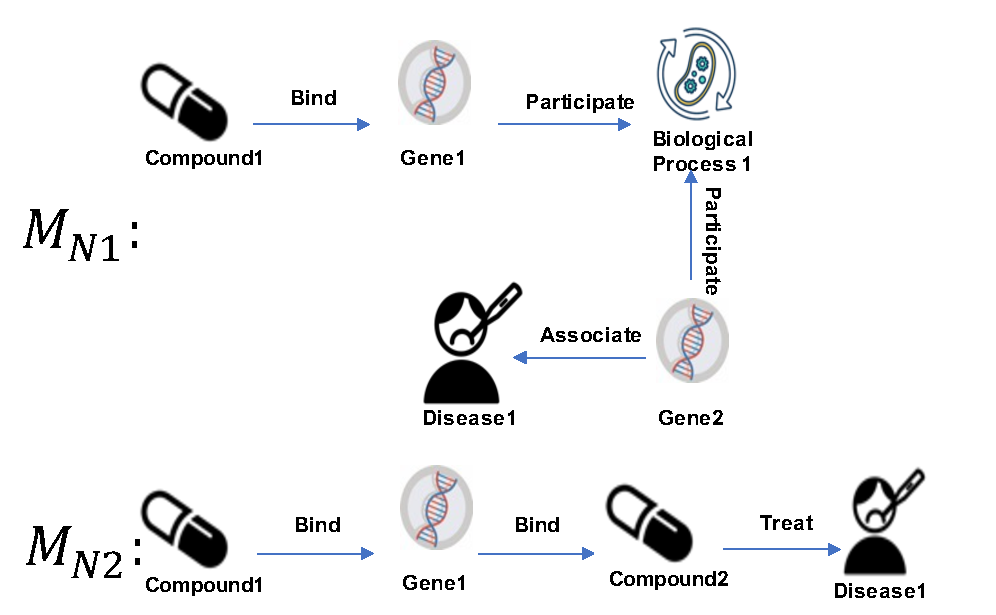
\includegraphics[width=0.8\linewidth]{./figures/decompose.pdf}
% \caption{Two meta paths decomposed from the meta structure $M_N$ in Fig.~\ref{fig:tabular}.}
% \label{fig:decompose}
% \end{figure}
% \begin{equation}
% \label{eq:decompose_meta_path}
% \begin{aligned}
% M_{N_1}:Compound1 \stackrel{Bind}{\longrightarrow}Gene1\stackrel{Participate}{\longrightarrow} Biological Process1 \stackrel{Participate}{\longleftarrow} Gene2\stackrel{Associate}{\longrightarrow} Disease1 \\
% M_{N_2}:Compound1 \stackrel{Bind}{\longrightarrow}Gene1\stackrel{Upregulate}{\longrightarrow} Compound1 \stackrel{Treat}{\longleftarrow}Disease1.
% \end{aligned}
% \end{equation}
% $M_{N_1}:Compound1 \stackrel{Bind}{\longrightarrow}Gene1\stackrel{Participate}{\longrightarrow} Biological Process1 \stackrel{Participate}{\longleftarrow} Gene2\stackrel{Associate}{\longrightarrow} Disease1$ and $M_{N_2}:Compound1 \stackrel{Bind}{\longrightarrow}Gene1\stackrel{Upregulate}{\longrightarrow} Compound1 \stackrel{Treat}{\longleftarrow}Disease1$.
% \item[2)]  There are many well-studied path finding algorithms, which can search the paths under different types of constraints, such as Dijkstra’s algorithm~\cite{lanning2014dijkstra}, A* search~\cite{cui2011based}, best-first search~\cite{heusner2018best}, etc.
% These off-the-shelf methods can be directly adopted to our framework.
% In the experiments, we adopt the best-first search algorithm.
% \item[3)] Lots of existing rule mining methods~\cite{sadeghian2019drum,yang2017differentiable,ho2018rule} designed for the \textit{closed rules}, meaning that each entity set appears in at least two edges of the rule.
% It renders the path-like graph structure in most cases.
% \end{itemize}
So we find all the candidate causes by searching all the paths between entity pairs $(x, y)$, which have the relation $R_h$ between them.
There are many well-studied path finding algorithms, which can search the paths under different types of constraints, such as Dijkstra’s algorithm~\cite{lanning2014dijkstra}, A* search~\cite{cui2011based}, best-first search~\cite{heusner2018best}, etc.
% These off-the-shelf methods can be directly adopted to our framework.
In the experiments, we adopt the best-first search algorithm.
Since the number of candidate causes can be the power level of the number of relation types, we require that the length of the path is no more than $\ell$, where $\ell$ is the hyper-parameters.
In the experiments of this paper, we set $\ell$ as 3.
% need to be supported by at least $a_{sup}$ entity pair $(e^h,e^t)$ in the training KG, and the length of the path is no more than $\ell$, where $a_{sup}$ and $\ell$ are the hyper-parameters.
(2) Step-2: generating samples.
% In tabular data, variables have distinct physical meanings, and the values of each instance are accessed via data collection.
% There is no explicit quantitative information inside triple-based knowledge graphs.
% For further causality learning, the assignment rules for the variables specified by structural attributes must be agreed upon in order to generate a numerical sample set that can be statistically analyzed.
In this paper, we use the connectivity as the assignment function to get quantitative samples.
\noindent
\begin{definitionnew} the
\textbf{binary assignment function of rule-induced variable} is as following:
$$
f_\mathcal{G}(e_h,e_t|\mathbf{R_b}^k)=\mathbbm 1_{\rm con}(e_h,e_t|\mathbf{R_b}^k)
$$
where $\mathbbm 1_{\rm con}(e_h,e_t|\mathbf{R_b}^k) \in \{0,1\}$ checks whether there exists a path instance of $\mathbf{R_b^k}$ between $e_h$ and $e_t$ in KG $\mathcal{G}$.
\end{definitionnew}

% \begin{definition} the
% \textbf{binary assignment function of meta structural attribute-defined variable} is as following:
% $$
% f_{\mathcal{G},(C_h,C_t).M}(e_h,e_t)=\left\{
% \begin{aligned}
%     1  & \text{~~if condition one is satisfied}. \\
%     0 & \text{~~otherwise}.
% \end{aligned}
% \text{for~} e_h \in
%     \mathcal{E}_h \text{~and~} e_t \in \mathcal{E}_t\\
% \right.
% $$
% where condition one is there is an meta structure instance of $M$ between $e_h$ and $e_t$ in KG $\mathcal{G}$.
% \end{definition}

In this assignment function, we consider whether two entities can be connected via a relation path, instead of the entities or number of the connection paths.
There are two main reasons for this design:
(1) We expect that the mined causal relationship can be generalized to any dataset in this domain.
% Without the attribute of the entities, we can not model the entities based on the their common features.
Thus, if we want to distinguish different entities which instantiate the meta structure, we need to build a multinomial model for all possible entities.
The multinomial would be infeasibly large.
And our model can not be applied to any scenario which contain an unseen entity.
(2) this function can be seen as an aggregation function to summary the connection information between entities.
The aggregation function is very common in the causal relation model~\cite{maier2010learning,lee2016learning,lee2020towards,salimi2020causal}.
With the aggregation function, we can build a concise and expressive model.
Since the only thing we need is whether the entities are connected.
Based on this assignment function, by sampling entity pairs in the training KG and querying the corresponding variable values, we can obtain tabular data for causal analysis.




% (2) Step-2: Refinement of the Identical Relations.
% In KG, there may be some identical relations, even though they have different relation names.
% For example, Wife(A,B) $\leftrightarrow$ Husband(B,A), if A is the wife of B, then B must be the husband of A.
% However, they will lead the invalid independence test in the following causal discovery step, even though these two relations have very strong causal relationship with each other.
% In particular, based on the causal variable and sample definitions in KG (Sec.~\ref{sec:v_a_s}), these two relations are the same variables for the causal discovery method, since the values of their samples are the same all the time.
% When one relation is treated as the conditional variable in the independent test of the other one, the conditional independence (CI) test $CI(X,Y|X)$ will be judged as independent.
% So for an analyzed KGS $S_E$, we search all the identical KGSs in the input KG and temporarily remove them from the candidate cause set in the independent test period.
% The causal rules which include the identical KGSs will have the highest weight, when they are applied into the downstream tasks.
\subsection{Causal MetaKnowlege Discovery via $d$-seperation Criterion}
\label{sec:discovery}

The $d$-separation criteria~\cite{glymour2016causal} (see Definition 3.4) is a sufficient and necessary condition for the compatibility of a probability distribution with a causal model in the form of a directed acyclic graph (DAG).
It states that a joint probability distribution of a set of random variables is compatible with the DAG (each node represents one of the given variables and each arrow represents the possibility of causal influence) if and only if the distribution satisfies a set of conditional independence relations encoded in the structure of the DAG.
Therefore, $d$-separation is widely used in the algorithms in discovering causal structure\cite{giudice2022dual,sondhi2019reduced,gerhardus2020high}.

\begin{definitionnew}
\textbf{d-seperation.} A path $p$ is blocked by a set of nodes $Z$ if and only if:

1.$p$ contains a chain of nodes $A \to B\to C$ or a fork $A \gets B\to C$ such that the middle node $B$ is in $Z$ (i.e., $B$ is conditioned on), or:

2. $p$ contains a collider $A \to B \gets C$ such that the collision node $B$ is not in $Z$, and no descendant of $B$ is in $Z$.

If $~Z$ blocks every path between two nodes $X$ and $Y$, then $X$ and $Y$ are $d$-separated, conditional on $Z$, and thus are independent conditional on $Z$.
\end{definitionnew}


\begin{algorithm2e}
\caption{Local causal metaknowledge discovery}
\label{alg:pc-like}
\KwIn{$Y$ and $\{y_i\}, i=1,\dots,N$ : variable and samples of queried variable $(C_h,C_t).M_q$ ;
 $\mathcal{X}^{Ca} = \{X_k\}, k=1,\dots,K$ and $\{\{x_i\}_k\}, i=1,\dots,N$: variables and samples of candidate causes; }
\KwOut{causes $\mathcal{X}^{C}$ of $Y$}
level $d \gets 0$\;
\While{$d<= |\mathcal{X}^{Ca}|-1$}{

\For{each $X_k \in  \mathcal{X}^{Ca}$}{
    \For{each subset $\mathcal{Z} \in \mathcal{X}^{Ca} \backslash \{ X_k\}$ and $|\mathcal{Z}|=d$}{
    Test CI($X_k,Y|\mathcal{Z}$)\;
    \If{CI($X_k,Y|\mathcal{Z}$)}{
        Test CI($\mathcal{Z},Y|X_k$) {(Reverse CI test.)} \;
        \If{not CI($\mathcal{Z},Y|X_k$)}{
            Remove $X_k$ from $\mathcal{X}^{Ca}$\;
            Break\;
        }
    }
}
}
$d \gets d+1$\;
}
$\mathcal{X}^{C} = \mathcal{X}^{Ca}$
\end{algorithm2e}

In this work, we design an efficient causal metaknowledge discovery algorithm based on $d$-separation.
With $d$-separation, we can get the following conclusion: given any set of variables $Z$, where $Z$ does not include $X$, $X$ is not independent of its parent node ({i.e.} direct cause).
% \yym{theorem}
Based on this conclusion, we can obtain a criterion for determining the direct cause of variable $X$.
Furthermore, we design the following local causal metaknowledge discovery algorithm (Algo.~\ref{alg:pc-like}) for the queried variable $Y=f_{\mathcal{G}}(x,y|R_h)$.
We only mine the direct cause of $Y$, instead of the entire causal structure of variable set $\mathcal{X}^{Ca} \cup \{Y\}$.
Particularly, given a queried variable $Y=f_{\mathcal{G}}(x,y|R_h)$, for each candidate cause in $\mathcal{X}^{Ca}$~(denoted as variable $X_k$),
the proposed algorithm decides whether $X_j$ should be retained in candidate causes set $\mathcal{X}^{Ca}$ by testing the independence of $X_k$ and $Y$ conditioning on a subset $\mathcal{Z}$ of $\mathcal{X}^{Ca}\backslash \{X_k\}$.
The conditional independent(CI) tests are organised by levels (based on the size $d$ of the conditioning sets).
At the first level ($d = 0$), all pairs of variables are tested conditioning on the empty set.
Some of the candidate causes would be removed and the algorithm only tests the remaining candidate causes in the next level ($d = 1$).
The size of the conditioning set, $d$, is progressively increased (by one) at each new level until $d$ is greater than $|\mathcal{X}^{Ca}|-1$.
Each corresponding relation path of $X \in \mathcal{X}^C$ construct a valid rule to predict the relation $R_h$ in $Y$.

\begin{figure}[t]
\vspace{0cm}
\centering
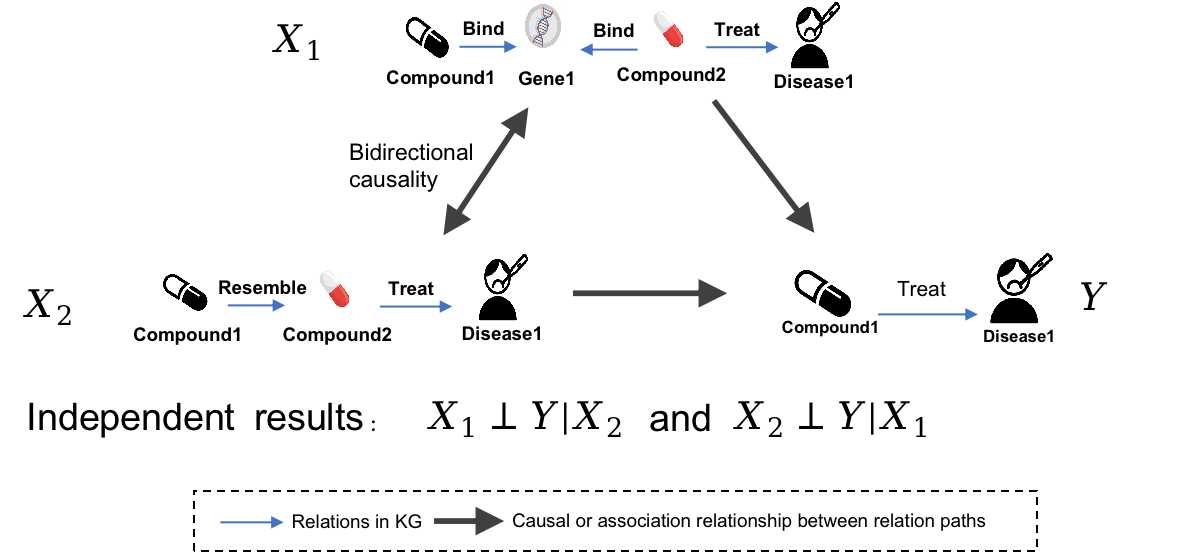
\includegraphics[width=8.5cm]{submissions/causal-meta-knowledge/figures/bidirection.jpg}

\caption{An example of bidirectional causal relationship, which may lead wrong results.}
\label{fig:bidirection}

\end{figure}

It is noteworthy that we add the reverse CI test in Algo.~\ref{alg:pc-like} (line 7) to avoid the impact of redundant relations in KGs.
For example, $Compound1 \stackrel{Resembles}{\longrightarrow}Compound2$ and $Compound1 \stackrel{Binds}{\longrightarrow}Gene1\stackrel{Binds}{\longleftarrow}Compound2$ express the similar message, which could lead the invalid independence test, as shown in Fig.~\ref{fig:bidirection}.
% \xz{As shown in Fig. xx}, the CI test results
% $Y=(C_h,C_t).M_q  \perp  X_1=(C_h,C_t).M_1| X_2=(C_h,C_t).M_2$  and $Y\perp  X_2|X_1$, where $C_h$ is Compound1, $C_t$ is Disease1, $M_q=Compound1 \stackrel{Treats}{\longrightarrow}Disease1$, $M_1= Compound1 \stackrel{Resembles}{\longrightarrow}Compound2 \stackrel{Treats}{\longrightarrow}Disease1$ and  $M_2= Compound1 \stackrel{Binds}{\longrightarrow}Gene1\stackrel{Binds}{\longleftarrow}Compound2 \stackrel{Treats}{\longrightarrow}Disease1$.
It will lead both $X_1$ and $X_2$ are removed from the candidate cause set of queried variable $Y$, even though they have very strong causal relationship with the drug treatment of diseases.
Consequently, we use the reverse CI test to avoid this issue.
In particular, if $X_j$ and $Y$ are judged to be independent conditioning on $\mathcal{Z}$, we will examine the independence between $\mathcal{Z}$ and $Y$ conditioning on $\mathcal{X}_j$.
When the result of the additional test is negative, $X_j$ will be removed from $\mathcal{X}^{Ca}$.
In this paper, we adopt SCI method~\cite{marx2019testing} as the independent test method in the experiments, which works well on limited samples and discrete variables.

\subsection{Link Prediction based on Explainable Causal Metaknowledge}
\label{sec:link_pred}

The approach for link prediction based on interpretable rules tends to generate corresponding weights in the rule mining phase. By accumulating the weights of the rules satisfied by each predicted entity, a score of the predicted entities can be generated, and then the results are ranked based on this score.
Here we first introduce how to generate rule weights under the causal model and then describe the approach for link prediction based on generated weights.

\begin{figure}[t]
\vspace{0cm}
\centering
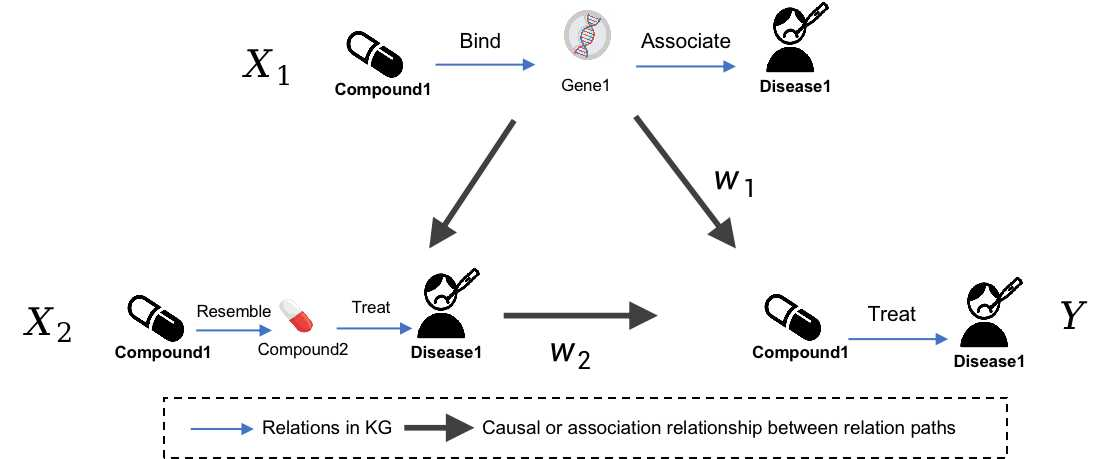
\includegraphics[width=8.5cm]{submissions/causal-meta-knowledge/figures/direct_cause.jpg}
% \vspace{-3pt}
\caption{An example of non-independent rule-induced variables, which are both the causes of queried relation.}
\label{fig:direct_cause_example}
% \vspace{-5pt}
\end{figure}

\noindent
\textbf{Weights of rules based on conditional dependency.}
In Algo.~\ref{alg:pc-like}, we discover the direct causes by the non-independence relationship between the candidate meta structures and the queried meta structures.
It is important to note that the meta structures of $\mathcal{X}^C$ are not independent to each other.
Fig.~\ref{fig:direct_cause_example} gives an example for this case. Specifically, $X_1$ and $X_2$ are both causes of $Y$.
Since $X_1$ is also a cause of $X_2$, if we directly calculate the causal strength between $X_2$ and $Y$, it is inevitable that $w_2$ will contain the causal effects that arise from $X_1$ along the path $X_1\to X_2 \to Y$.
Therefore, in order to better measure the importance of each causal rule and to avoid double-counted in the calculation of each proposed entity's score, we adopt the minimal conditional dependence as a measure of the importance of causal rules:

\begin{equation}
\label{eq:weight}
\begin{aligned}
w_j  = \min(\{ dependence(X_j,Y|\mathcal{Z}) \})
\\
\text{~for any subset~} \mathcal{Z} \in \mathcal{X}^{Ca}\backslash \{X_j\},
\end{aligned}
\end{equation}
where $w_j$  is the rule weight of the meta structure in $X_j$.
In this paper, we use the $SCI_f(X,Y|Z)$ in SCI independence test~\cite{marx2019testing} as the dependence score in Eq.~\ref{eq:weight}, which can be get in the process of causal rules discovery.
The higher of $SCI_f(X,Y|Z)$, the stronger the dependency.

\noindent
\textbf{Score function of entity results.}
Because of the incompleteness nature of KGs, open world assumption (OWA)~\cite{ji2021survey} is often considered on real datasets.
Under the OWA, the SUM function are usually adopted to calculate the ranking score of the predicted entity $e_h$ in link prediction task $(?,R_h,e_t)$:
\begin{equation}
\label{eq:link-prediction-sum}
\begin{aligned}
S_{R_q}^{sum}=\sum_{i=1}^K \tilde{w}_i Q_{i},.
\end{aligned}
\end{equation}
where $K$ is the number of causal rules, $\tilde{w}_i$ is the normalized weight.
$Q_i=1$ when the body of the $i$-th causal rule holds for the entity pair ($e_h, e_t$), otherwise $Q_i=0$.
This approach focuses on the entities supported by multiple rules and does not use the non-existent relations between entity pairs, since the unreliable negative samples under OWA.
In this paper, Eq.~\ref{eq:link-prediction-sum} is used in the link predictions on real data.
For KG under closed world assumption(CWA)~\cite{ji2021survey}, the negative facts are also reliable, therefore we design a new function to apply the rules in the link prediction task.
Particularly, given an query $(?,R_h,e_t)$, the score of the triple $(e_h,R_h,e_t)$ is true can be formulated as:
\begin{equation}
\label{eq:link-prediction-avg}
\begin{aligned}
S_{R_q}^{avg} = \sum_i^K \tilde{w}_i \big(Q_i \bar{Y}_{X_i=1} + (1-Q_i) \bar{Y}_{X_i=0}\big),
\end{aligned}
\end{equation}
where $K$ is the number of causal rules for the queried relation, $\tilde{w}_i$ is the normalized weight for the $i$-th result rule.
$\bar{Y}_{X_i=1}$ denotes the proportion of the queried relation to be true when the body of the $i$-th causal rule is true in the training data, and $\bar{Y}_{X_i=0}$ denotes the proportion of the queried relation to be true when the body of the $i$-th causal rule is false.
$Q_i=1$ when the body of the $i$-th causal rule holds for the entity pair ($e_h$, $e_t$), otherwise $Q_i=0$.
The results will be ranked by $S_{R_q}$ of each valid $e_t$.
In this paper, Eq.~\ref{eq:link-prediction-avg} is used in the link predictions on simulation data.


% For the link prediction $<?,R,e_t>$, there are two ways to calculate the ranking score of the predicted entity $e_h$:
% \begin{itemize}
% %     \item MAX: this approach highlights the role of the highest-impact rule.
% % \begin{equation}
% % \label{eq:link-prediction-max}
% % \begin{aligned}
% % S_{R_q}^{max}=\max \left\{\tilde{w}_{1} Q_{1}, \tilde{w}_{2} Q_{2}, \ldots, \tilde{w}_{K} Q_{K}\right\}.
% % \end{aligned}

%  \item SUM: this approach focuses on the results supported by multiple rules.
% \begin{equation}
% \label{eq:link-prediction-sum}
% \begin{aligned}
% S_{R_q}^{sum}=\sum_{i=1}^K \tilde{w}_i Q_{i},.
% \end{aligned}
% \end{equation}
% where $K$ is the number of causal rules, $\tilde{w}_i$ is the normalized weight.
% $Q_i=1$ when the body of the $i$-th causal rule holds for the entity pair ($e_h, e_t$), otherwise $Q_i=0$.
% \item AVG: \xz{for a $e_t$, this approach considers both the prediction of a rule on the target relation when it is satisfied and unsatisfied.}

% \begin{equation}
% \label{eq:link-prediction-avg}
% \begin{aligned}
% S_{R_q}^{avg} = \sum_i^K \tilde{w}_i \big(Q_i \bar{Y}_{X_i=1} + (1-Q_i) \bar{Y}_{X_i=0}\big),
% \end{aligned}
% \end{equation}
% where $\bar{Y}_{X_i=1}$ denotes the proportion of the queried relation to be true when the body of the $i$-th causal rule is true in the training data, and $\bar{Y}_{X_i=0}$ denotes the proportion of the queried relation to be true when the body of the $i$-th causal rule is false.
% \end{itemize}
% These ranking functions show their unique advantages under different application scenarios, and we provide thorough discussions for them based on the experimental results. 


\section{Experimental Study}
\label{section:experiment}
\subsection{Experimental Setup}
In this section, we empirically evaluate the effectiveness and interpretability of the proposed~\dname~on both
simulation and real-world datasets.
For interpretability, we focus on whether the algorithm can uncover the causal relationships inherent in the knowledge graph.


\subsubsection{\textbf{Baselines}}
% The aim of this experiment was to evaluate both the effectiveness and interpretability of the existing methods and our approach.
% In this paper, we design a causal rule-based prediction algorithm mainly for application scenarios that require explainability.
To evaluate the interpretability of the algorithms, we select four rule-based methods
that can conduct link prediction and generate explainable rules.
To make a fair comparison, the inference rules, obtained from different algorithms, are used to conduct the link prediction task based on the same prediction equations.
This approach can also help us observe the impact of different rules on the link prediction task.
For a complete evaluation of the effectiveness of the proposed approach, we also compute the LP performance of TuckER\cite{balazevic2019tucker}, one representation-based method which has the best overall performance among the representation-based methods across different datasets\cite{rossi2021knowledge}.
All baselines are listed in the following:
\begin{itemize}
\item[1)] AMIE+\cite{galarraga2015fast}, an efficient  top-down method to discover the interpretable rules.
\item[2)] AnyBURL\cite{meilicke2019anytime}, a bottom-up approach to mine the logical rule.
\item[3)] Neural-LP\cite{yang2017differentiable}, an end-to-end differentiable model to learn the first-order logical rule.
\item[4)] RNNLogic\cite{qu2020rnnlogic}, an EM-based algorithm to learn the rule generator and the reasoning predictor iteratively.
\item[5)] TuckER\cite{balazevic2019tucker},  a linear model based on Tucker
decomposition of the binary tensor representation of knowledge graph triples.
\end{itemize}





\subsubsection{\textbf{Datasets}}
To quantitatively evaluate the effectiveness of the algorithm in discovering causal knowledge, we construct a simulation dataset owing to a lack of groundtruth of real datasets.
Douban and Hetionet~\cite{himmelstein2017systematic} are selected as our real datasets on which we perform two link prediction tasks, movie rating prediction and drug repurposing, respectively.
Here we provide more details for these datasets, and their statistics are shown in Table~\ref{tab:dataset_statistics}.

% \begin{figure}[t]
% \vspace{0cm}
% \centering
% 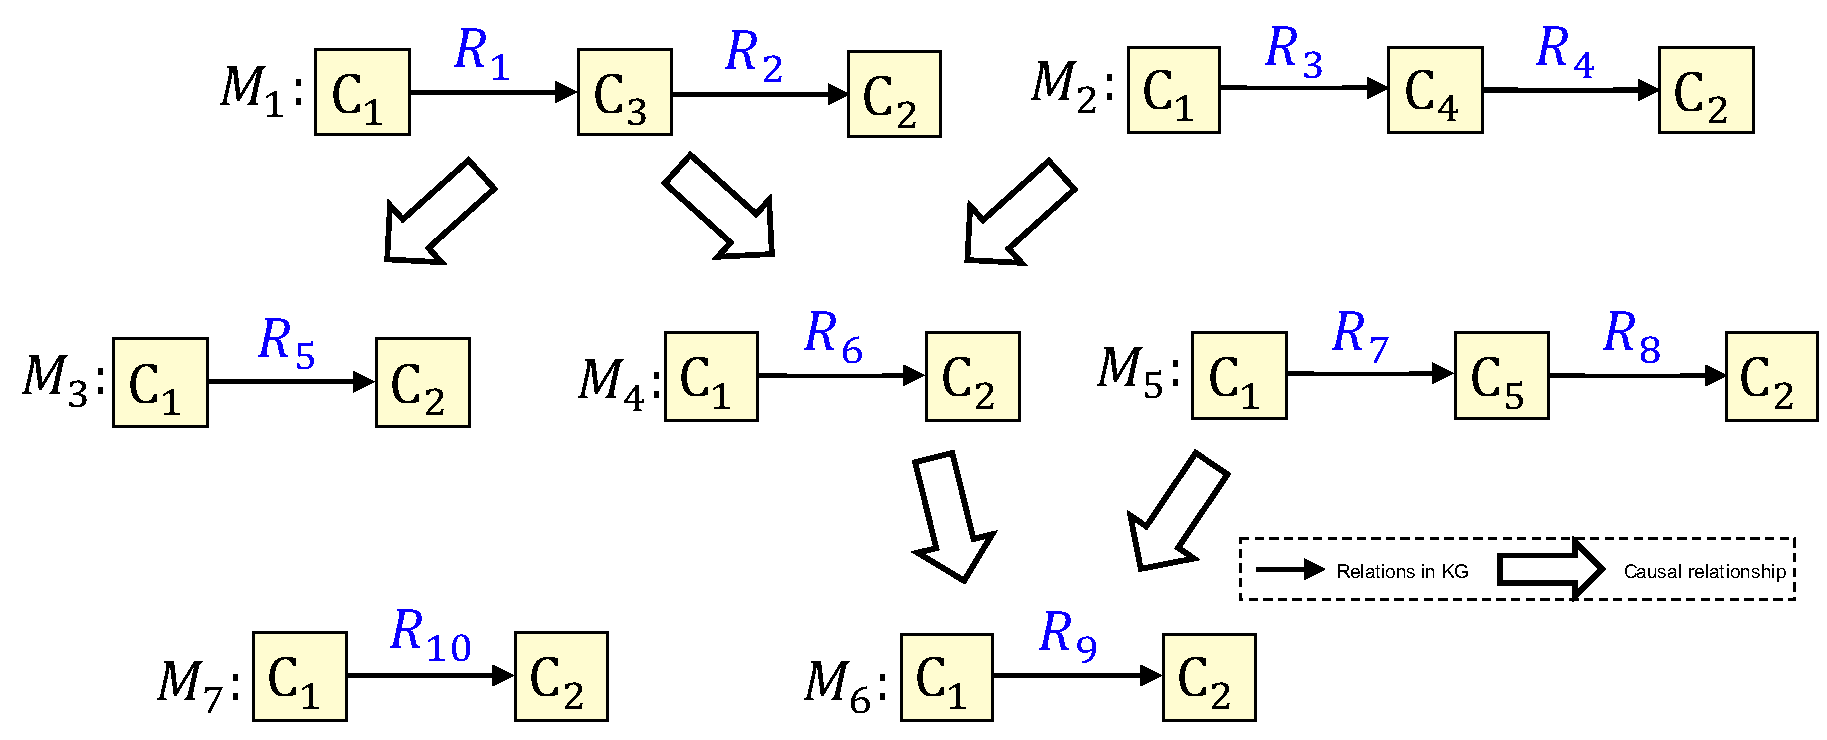
\includegraphics[width=8.5cm]{./figures/simulation.pdf}
% \caption{ The causal graph used to generate simulated knowledge graphs.}
% \label{fig:toy_example}
% \end{figure}

\begin{table}[t]
\centering
\caption{Dataset statistics of all the experiments.}
\label{tab:dataset_statistics}
% \vspace{-2pt}
\scalebox{1}{
\begin{tabular}{c|ccc}
\hline
   & \textbf{\#Triplets} & \textbf{\#Relations} & \textbf{\#Entities}  \\
\hline
\textbf{Simulation} & 6,095 & 5 & 1,590\\
\textbf{Douban Movie Rate} & 28,356 & 12 & 3,007 \\
\textbf{Hetionet} & 174,941 & 20 & 32,056 \\
\hline
\end{tabular}
}
\end{table}

\noindent
{\bf Simulation dataset.}
We generate simulated KGs based on a toy causal model specified in Fig.~\ref{fig:simulation}, which includes three concepts and five relations.
In particular, we design the causal mechanisms in KG via a probabilistic model.
The root nodes ($X_1$, $X_4$) in the causal graph are generated via Bernoulli distributions, whose probability mass function is $f_X(x)=p^x(1-p)^{1-x}$.
Moreover, the non-root nodes ($X_2$, $X_3$) are generated via the conditional probability distributions, which are Bernoulli distributions, given the parent node ($X_1$).
To maintain a stable causal mechanism, the parameters of conditional distributions are constant in training and testing, as shown in Table~\ref{tab:simulation_set}.
In the out-of-distribution paragraph, we will introduce the parameters of root nodes in training and testing.


\begin{figure}[h]
\centering
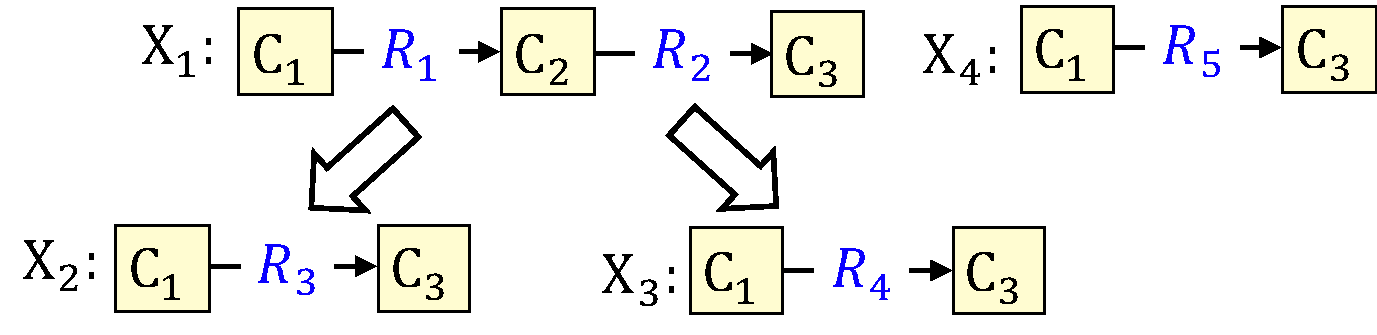
\includegraphics[width=7cm]{submissions/causal-meta-knowledge/figures/simulationv4.pdf}
\caption{The causal graph of relation paths, based on which the simulated KGs are generated .}
\label{fig:simulation}
% \vspace{-2pt}
\end{figure}

\begin{table}[h]
\caption{The parameters of conditional distributions.}
%\vspace{5pt}
\label{tab:simulation_set}
\centering
\scalebox{1}{
\begin{tabular}{c|cccc}
\hline
Conditions & $X_2|X_1=1$ & $X_2|X_1=0$ & $X_3|X_1=1$ & $X_3|X_1=0$ \\
\hline
Parameters & $p$=0.9 & $p$=0.1 & $p$=0.9 & $p$=0.1 \\
\hline
\end{tabular}}
% \vspace{-2pt}
\end{table}
% We generate simulated KGs based on a toy causal model specified in Fig.~\ref{fig:toy_example}, which includes five concepts and ten relations.
% More specifically, given $N$ entities for each concept, the facts containing the relations in the root nodes ($M_1$, $M_2$, $M_7$) of the causal graph are generated via Bernoulli distributions, whose probability mass function is $f(x)=p_r^x(1-p_r)^{1-x}$.
% For example, the entity pair $(e_1,e_3)$, where $e_1 \in \mathcal{E}_{C_1}$ and $e_3 \in \mathcal{E}_{C_3}$, the probability that the fact $<e_1,R_1,e_3> \in \mathcal{G}$ is $p_r$.
% % It means for any entity pair $(e_h,e_t)$, where $e_h \in \mathcal{E}_{C_h},\mathcal{E}_{C_t}$ and $R_i(C_h,C_t) \in \text{KG schema} \mathcal{S}$, the probability that the fact $R_i(e_h,e_t) \in \mathcal{T}$ is $p_r$.
% % we design the conditional  probabilistic distribution in SPRM based on which to sample the entity and facts in KG.
% And the facts in non-root nodes (e.g., $M_3$) are generated via the conditional probability distributions, which are Bernoulli distributions with parameter set $\mathbf{p}_{nr}$, given the facts information of parent node ($M_1$).
% For example, if there is a path instance of $M_1$ between $(e_1,e_3)$, then the probability of the existence of fact $<e_1,R_5,e_3>$ is $p_{M_1=1}$, otherwise is $p_{M_1=0}$.
% \yym{the value of all parameter of $p_nr$}

%


\noindent
{\bf Douban movie rating.}
Douban is a famous Chinese website for movie reviews, where users can rate and comment on any movie.
The rating range is from 1 to 5. A higher rating means that users like movies, while a lower rating means that users have negative feedback on movies.
We collect the real-world data from Douban\footnote{https://www.douban.com/} and construct a dataset (this dataset will be released), whose statistics are shown in Table~\ref{tab:dataset_statistics}.
Commonly, a movie with a score of 4 or 5 is identified as meeting the taste of users.
So we transform the original 5-level rating to a 2-level rating with a threshold of 4.
If the rating score is 4 or 5, the original relation \textit{Rate} is replaced by  \textit{HighRate}
We conduct the link prediction task on the relation \textit{HighRate}.
Because the raw data is too large and the relations between users and movies are very sparse, in this thesis, we first filter the 20 users who have made the most ratings and take the rating history of these users as the set of rating facts for our study.
The facts unrelated to the rating are also included in our experimental data.

\noindent
{\bf Hetionet}\cite{himmelstein2017systematic}
is a freely available knowledge database that integrates biomedical information from 29 prominent
bioinformatics resources.
Recently, Hetionet was successfully applied to drug repurposing tasks in terms of the link prediction task for relation \texttt{Treats}\cite{himmelstein2017systematic, ratajczak2022task}.

\textit{Why do we choose those two real datasets instead of other commonly used datasets, such as WN18, FB15k?}
In this paper, we focus on link prediction with the help of causal relationships between knowledge graph relations.
The core of causality lies in its asymmetry.
The commonly used KGs for link prediction algorithms contain many symmetrical relationships, e,g., \textit{hypernym} and \textit{hyponym} in WN18.
These symmetrical relationships may help with the link prediction task, but they go against the basic idea that causality is a one-way relationship.
We, therefore, chose datasets with specific application scenarios and rich causal semantics.

\subsubsection{\textbf{Metrics.}}
\textbf{For link prediction}, we employ the commonly used metrics mean reciprocal rank (MRR) and Hits@k~\cite{rossi2021knowledge,balazevic2019tucker,bordes2013translating}.
\begin{equation}
\label{eq:mrr}
\begin{aligned}
M R R=\frac{1}{|Q|} \sum_{q \in Q} \frac{1}{q}
\end{aligned}
\end{equation}

\begin{equation}
\label{eq:hitk}
\begin{aligned}
Hit@K=\frac{|\{q \in Q: q \leq K\}|}{|Q|}
\end{aligned}
\end{equation}
where $Q$ is the rank results, for each $q_i \in Q$ is the ranking of the desired results in the $i$-th query $(?,R_h,e_t)$.
In the case of ties in the calculation of $Q$, we use the mean rank to avoid misleading results\cite{rossi2021knowledge,ruffinelli2020you}.
% Common values for $K$ are 1, 3, 5, 10, we use $K=5$ in this paper.
Both MRR and His@k are the higher, the better.

\noindent
\textbf{The interpretability of causal rules} on the simulation dataset can be understood as the consistency between the mined causal rules and the actual causal structure.
Therefore, we evaluate baselines and our approach on the simulation dataset using precision, recall, and structural Hamming distance (SHD) as the evaluation metrics, which are commonly used evaluation metrics in causal structure discovery studies~\cite{zheng2018dags,zheng2020learning}.
% Since the performance of causal rule discovery is the foundation of our link prediction method.

\begin{equation}
\label{eq:precision}
\begin{aligned}
Precision=\frac{\# TFR}{\#FR};Recall=\frac{\# TFR}{\#ATR}
\end{aligned}
\end{equation}
Where $\#TFR$ is the number of right causal relationships discovered by an algorithm, $\#FR$ is the number of causal relationships discovered by an algorithm, and $\#ATR$ is the number of all causal relationships.
Both precision and recall are the higher, the better.
SHD calculates the difference between the learned graph and the ground truth graph by the number of edge insertions, deletions, or flips required to transform one graph into another.
The lower the SHD, the better.

\subsubsection{\textbf{Out-of-Distribution Link Prediction}}
Traditional machine learning methods are designed based on the assumption of independent and identically distributed (I.I.D) data.
This assumption means the training and test data come from the same distribution. However, the distribution of test data may alter due to changes in the test environment; such tasks are referred to as OoD tasks.
Traditional algorithms perform poorly on generalization problems due to the violation of I.I.D assumption.
Causality is seen as a stable inference mechanism in many research works on generalization problems.
So, in this work, we provide an out-of-distribution generalization task for the knowledge link prediction task for the first time.
On the one hand, the effect of causal metaknowledge on this task can be measured, and on the other, the performance of existing algorithms can be looked at.
We also evaluate the performance of the algorithms on I.I.D link prediction tasks.

In this paper, we design two OoD experimental scenarios.

\noindent
(1) \textit{Simulation dataset}:
We evaluate the link prediction performance under I.I.D and OoD settings, where the triples of root node $X_1$ are generated in testing under the same and different parameters with training.
In the training and I.I.D testing datasets, $p_{X_1}=0.5$.
In the OoD testing datasets, $p_{X_1} \in \{0.2,0.9\}$.
For $X_4$, $p_{X_4}$ maintains $0.9$ in training and testing.
The facts of the KGs are split into three parts:\textit{train}, \textit{test info}, and \textit{test}.
The facts in \textit{train} are used to learn the rule.
The effectiveness of the learned rule is assessed via the link prediction task on $R_3$.
The \textit{test info} part includes facts of new entities (did not appear in \textit{train}) on $R_1, R_2, R_4, R_5$, and \textit{test} part includes the queried facts on $R_3$.

\noindent
(2)\textit{Real datasets}:
It is impossible to explicitly change the data distribution since real data distribution is inaccessible for real datasets.
Recent research\cite{tang2020investigating,wu2021self} has suggested that graph models are biased towards nodes with larger degrees, which causes the bad performance of low-degree nodes in the test.
Therefore we construct the OoD datasets based on degree shift.
Specifically, given a query task $(?,R_h,e_t)$, we calculate the \textit{median} of degree\footnote{In this paper, we use the term "degree" to stand for the sum of in and out degrees} of known entities $e_t$ belonging to the triples $(e_h,R_h,e_t)$ in the training.
Then we bin the test queries by the degrees of the known entities $e_t$.
The degree range in each bucket is decided based on the sample size balance.
The test queries in the bucket, which the training median falls in, can be treated as the I.I.D test samples.
Others are the OoD samples.
The I.I.D bucket is labeled with $*$ in Table~\ref{tab:douban-mrr} and Table~\ref{tab:hetionet-mrr}.





\subsection{Performance of Link prediction task in Out-of-Distrition Settings}

\noindent
\textbf{Results on simulations.}
For the simulation dataset, we construct a OoD setting named as covariance shift, by changing the probability distribution of the root nodes in the test phase.
Table~\ref{tab:simulation_result} presents the methods in performance and demonstrates the effectiveness of the proposed \dname.
In particular, \dname~outperforms the baseline models under all metrics except the Hits@10 under I.I.D setting. This shows our method can give a stable and high-quality result, especially in the OOD setting.
Besides, compared with the baselines, the proposed \dname~ perform significantly better at the Hits@1 metric (at least 25\% absolute improvements that the second place under all settings), which suggests the our method are more suitable for scenarios with strict performance requirements, and this feature may achieved by the removal of association-based rules.

\begin{table}[h]
\caption{The results of link prediction on simulation datasets.}
\centering
\label{tab:simulation_result}
\scalebox{1.2}{
\begin{tabular}{c|c|l|cccc}
\hline
 \multirow{2}{*}{\textbf{Settings}}& \multirow{2}{*}{$\mathbf{p_{X_1}}$} & \multirow{2}{*}{\textbf{Method}} & \multirow{2}{*}{\textbf{MRR}} & \multicolumn{3}{c}{\textbf{Hits}} \\ \cline{5-7}
& & & &\textbf{@10} & \textbf{@3} & \textbf{@1} \\ \hline
\multirow{4}{*}{I.I.D} & \multirow{4}{*}{0.5}
& AMIE+ & 0.87 & \textbf{98.99} & 94.95 & 78.79\\
&  & AnyBURL & 0.87 &\textbf{98.99}&94.95 &78.79\\
&  & Neural-LP &  0.80 & \textbf{98.99} & 92.42& 66.16\\
& & RNNLogic & 0.87 & \textbf{98.99} & 94.95 & 78.79\\
&& \dname & \textbf{0.94} & 98.48&\textbf{97.98} &\textbf{90.91}\\

 \hline
\multirow{4}{*}{OOD} & \multirow{4}{*}{0.2}
& AMIE+ & 0.875 & 96.91 & 93.81 & 81.44 \\
&  & AnyBURL &  0.875 & 96.91&93.81 & 81.44\\
& & Neural-LP & 0.68 & 98.97 & 79.38 & 50.51\\
& & RNNLogic & 0.875 & 96.91 & 93.81 & 81.44 \\
&& \dname & \textbf{0.99} & \textbf{100}&\textbf{100} &\textbf{99.97}\\
 \hline
 \multirow{4}{*}{OOD} & \multirow{4}{*}{0.9}
& AMIE+ & 0.91 & \textbf{100} & 96.34 & 85.67 \\
&  & AnyBURL &  0.91 &\textbf{100} & 96.34 & 85.67\\
& & Neural-LP & 0.88 & \textbf{100} & 96.95 & 79.57\\
& & RNNLogic & 0.91 & \textbf{100} & 96.34 & 85.67 \\
&& \dname & \textbf{0.99} &  \textbf{100}& \textbf{99.70} & \textbf{99.09}\\
 \hline
\end{tabular}
}
\end{table}

% Also we considered the effect of different score functions on the link prediction performance.
% The results are shown in Tab.~\ref{tab:simulation_result}, and  can find that our method also works well for the simulated data, especially under OoD settings. Specifically, our model gets the best MRR and Hit@1 results, while AMIE+ and AnyBURL are the best methods for Hit@5 and Hit@10 for I.I.D setting. This may be because they tend to discover more rules, while our method aims to identity the causality more accurately, so fewer links are predicted.
% For OoD data, the proposed method surpasses all baseline models on all metrics, which fully support our motivation: building a link prediction algorithm with strong generalization ability.

% Overall, our method performs best for all three datasets. Also note although some baselines get the best results under some specific settings, they can not maintain a good performance for other settings or metrics. For example, TuckER gets the best MRR under 0-5 degree range, while performs worst with 30-60 degree range on Douban movie rating dataset. By contrast, the proposed CMLP can achieve best or competitive results for all settings.

% \yym{Prior systems for generating conjectures have either contributed genuinely useful research conjectures9 via methods that do not easily generalize to other mathematical areas10, or have dem- onstrated novel, general methods for finding conjectures11 that have not yet yielded mathematically valuable results.}


% \begin{table}[h]
% \caption{The results of link prediction on simulation datasets.}
% \centering
% \label{tab:simulation_result}
% \scalebox{1}{
% \begin{tabular}{c|c|l|cccc}
% \hline
%  \multirow{2}{*}{\textbf{Settings}}& \multirow{2}{*}{$\mathbf{p_{r}}$} & \multirow{2}{*}{\textbf{Method}} & \multirow{2}{*}{\textbf{MRR}} & \multicolumn{3}{c}{\textbf{Hits}} \\ \cline{5-7}
% & & & &\textbf{@1} & \textbf{@5} & \textbf{@10} \\ \hline
% \multirow{5}{*}{I.I.D} & \multirow{5}{*}{0.3}
% & AMIE+ & 0.734 & 0.589 & \textbf{0.948} & \textbf{1}\\
% &  & AnyBURL & 0.733 & 0.589 & \textbf{0.948} & \textbf{1}\\
% &  & Neural-LP &  0.58 & 0.41 & 0.743 & 0.769\\
% &  & RNNLogic &  0.603 & 0.461 & 0.666 & 0.666\\
% & & \dname & \textbf{0.785} & \textbf{0.692} & 0.897 & 0.897 \\

% %  \hline
% % \multirow{5}{*}{OOD} & \multirow{5}{*}{0.1}
% % & AMIE+ & 0.73 & 0.538 & \textbf{0.846} & \textbf{0.846} \\
% % &  & AnyBURL &  \textbf{0.782} & \textbf{0.615} & \textbf{0.846} & \textbf{0.846} \\
% % & & Neural-LP & 0.673 & 0.461 & 0.769 & 0.769\\
% % & & RNNLogic & 0.611 & 0.307 & 0.538 & 0.538\\
% % && \dname & 0.692 & 0.538 & 0.692 & 0.692\\
%  \hline
%  \multirow{5}{*}{OOD} & \multirow{5}{*}{0.8}
% & AMIE+ & 0.891 & 0.843 & \textbf{0.98} & \textbf{1} \\
% &  & AnyBURL &  0.893 & 0.843 & \textbf{0.98} & \textbf{1}\\
% & & Neural-LP & 0.885 & 0.843 & 0.941 & 0.98\\
% & & RNNLogic & 0.853 & 0.803 & 0.882 & 0.882\\
% && \dname & \textbf{0.909} &  \textbf{0.862} & \textbf{0.98} & \textbf{1}\\
%  \hline
% \end{tabular}
% }
% \end{table}
\noindent
\textbf{Results for Douban movie rating.}
Since we filtered the users of the Douban data, and the discrepancies of the degrees of experimental user nodes are close to each other.
Therefore, in this experiment, to construct the OoD scenario, we adopt the head prediction (? , HighRate, Movie), predicting the set of users who gave high ratings to movies.
Further, we bucketed the movie nodes in the test data according to their degree in the training data to observe the performance of the algorithm under different node prevalence.
The MRR and Hits@5 results shown in
Tab.~\ref{tab:douban-mrr} shows that the proposed CMLP get the best performance in the all OoD settings.
Especially, at least 25.8\% and 29.3 \% relative improvements that the second place on the MRR and Hits@5, respectively.
In the I.I.D setting, ~\dname~gets the second place on both MRR and Hits@5, lower than the representation-based method TuckER.
These results illustrate that for movie
rating datasets, the rules learned by our method can capture more general user preferences and give relatively accurate rating predictions for movies that are in different popularity.





% sum query head
\begin{table}[]
\centering
\caption{MRR (left) and Hits@5 (right) for Douban movie rating. The * marks columns that contain the I.I.D results. Other columns contain OoD results.}
\label{tab:douban-mrr}
\scalebox{1.2}{
\begin{tabular}{c|ccccc}
\hline
\multirow{2}{*}{\textbf{Methods}} & \multicolumn{4}{c}{\textbf{Degree Range}} \\ \cline{2-5}
          & \textbf{0-21*}   & \textbf{21-31}   & \textbf{31-39} & \textbf{39-60} \\ \hline
AMIE+     & 0.120 & 0.205 & 0.261 & 0.395 \\
AnyBURL   & 0.125 & 0.182  & 0.231 & 0.373 \\
Neural-LP & 0.078 & 0.097  & 0.126 & 0.217 \\
RNNLogic  & 0.072 & 0.086  & 0.097 & 0.161 \\
TuckER    & \textbf{0.287} & 0.186  &  0.186 & 0.149 \\
\dname      & 0.251 & \textbf{0.343}  & \textbf{0.392} & \textbf{0.497}\\ \hline
\end{tabular}
\quad
\begin{tabular}{c|ccccc}
\hline
\multirow{2}{*}{\textbf{Methods}} & \multicolumn{4}{c}{\textbf{Degree Range}} \\ \cline{2-5}
         & \textbf{0-21*}    & \textbf{21-31}   & \textbf{31-39} & \textbf{39-60}  \\ \hline
AMIE+        & 13.7 &30.7  & 39.4  & 68.3  \\
AnyBURL      & 15.1  & 26.0  & 33.2 & 64.6  \\
Neural-LP    & 0.1      & 0.6     & 3.4     & 60.0 \\
RNNLogic     & 1.6    & 4.7  & 7.2 & 13.5  \\
TuckER     & \textbf{50.3}   & 31.9   & 28.2  &  21.5 \\
\dname     & 40.9  & \textbf{60.0}  & \textbf{68.1} & \textbf{88.3}  \\ \hline
\end{tabular}}
\end{table}


% \begin{table}[]

% \caption{Hits@5 for Douban movie rating. The * marks columns that contain the I.I.D results. Other columns contain OoD results.}
% \label{tab:douban-hits1}
% \begin{tabular}{c|ccccc}
% \hline
% \multirow{2}{*}{\textbf{Methods}} & \multicolumn{4}{c}{\textbf{Degree Range}} \\ \cline{2-5}
%          & \textbf{0-21*}    & \textbf{21-31}   & \textbf{31-39} & \textbf{39-60}  \\ \hline
% AMIE+        & 13.7 &30.7  & 39.4  & 68.3  \\
% AnyBURL      & 15.1  & 26.0  & 33.2 & 64.6  \\
% Neural-LP    & 0.1      & 0.6     & 3.4     & 60.0 \\
% RNNLogic     & 1.6    & 4.7  & 7.2 & 13.5  \\
% TuckER     & \textbf{50.3}   & 31.9   & 28.2  &  21.5 \\
% \dname     & 40.9  & \textbf{60.0}  & \textbf{68.1} & \textbf{88.3}  \\ \hline
% \end{tabular}
% \end{table}

\noindent
\textbf{Results for drug repurposing on Hetionet.}
Consistent with the traditional setup of drug redirection, on Hetionet, we also use head predition (?, Treat, Disease), which is giving a Disease to predict new drugs. We also observe the performance of the algorithm under this task by bucketing for Disease node degrees.
Tab.~\ref{tab:hetionet-mrr} reports the MRR and Hits@5 on this dataset, and we can find that: our CMLP performs significantly better than other baselines on low-degree diseases (0-17), while AMIE+ and AnyBURL get better results on low-degree diseases (17-100).
These results indicate that our method can give more accurate drug discovery results for diseases with relatively low information.
And for diseases with richer information, the correlation-based inference rules give more accurate drug prediction.


\begin{table}[]
\centering
\caption{MRR(left) and Hits@5(right) for drug repurposing on Hetionet. The * marks columns that contain the I.I.D results. Other columns contain OoD results.}
\label{tab:hetionet-mrr}
\scalebox{1.2}{
\begin{tabular}{c|ccccc}
\hline
\multirow{2}{*}{\textbf{Methods}} & \multicolumn{4}{c}{\textbf{Degree Range}} \\ \cline{2-5}
    & \textbf{0-8*}    & \textbf{8-17}   & \textbf{17-31}  & \textbf{31-100} \\ \hline
AMIE+   & 0.103  & 0.085  & \textbf{0.132}  & 0.065 \\
AnyBURL  & 0.116   & 0.189  & 0.090  & \textbf{0.188} \\
Neural-LP & 0.027  & 0.014  & 0.009  & 0.009 \\
RNNLogic & 0.07  & 0.021  & 0.029  & 0.012 \\
TuckER  &  0.044  & 0.022    & 0.083   &  0.015 \\
\dname  & \textbf{0.248}  & \textbf{0.208}  & 0.095 & 0.093 \\ \hline
\end{tabular}
\quad
\begin{tabular}{c|cccc}
\hline
\multirow{2}{*}{\textbf{Methods}} & \multicolumn{4}{c}{\textbf{Degree Range}} \\ \cline{2-5}
  & \textbf{0-8*}    & \textbf{8-17}   & \textbf{17-31}  & \textbf{31-100} \\
  \hline
AMIE+      & 13.2  & 11.3  & \textbf{22.5} & 13.2  \\
AnyBURL     & 15.8  & \textbf{25.0}  & 9.6  & \textbf{23.7}   \\
Neural-LP   & 5.3      & 0     & 0      & 0      \\
RNNLogic  & 7.9  & 0  & 3.2      & 0      \\
TuckER    &  3.1   & 5.9  &  10.7  &  3.2   \\
\dname     & \textbf{26.31}  & \textbf{25.0} & 16.1 & 13.1  \\ \hline
\end{tabular}}
\end{table}

% \begin{table}[]

% \caption{MRR for drug repurposing on Hetionet. The * marks the range in which the mean of the training data falls.}
% \label{tab:hetionet-mrr}
% \begin{tabular}{c|ccccc}
% \hline
% \multirow{2}{*}{\textbf{Methods}} & \multicolumn{3}{c}{\textbf{Degree Range}} \\ \cline{2-4}
%     & \textbf{0-5}    & \textbf{5-15*}   & \textbf{15-30}   \\ \hline
% AMIE+   & 0.277  & 0.103  & 0.126   \\
% AnyBURL  & 0.28   & 0.177  & 0.134  \\
% Neural-LP & 0.036  & 0.016  & 0.011  \\
% RNNLogic & 0.149  & 0.038  & 0.023   \\
% TuckER  &  0.085  & 0.021    & 0.078    \\
% \dname  & \textbf{0.329}  & \textbf{0.327}  & \textbf{0.261} \\ \hline
% \end{tabular}
% \end{table}

% \begin{table}[]

% \caption{Hits@5 for drug repurposing on Hetionet. The * marks columns that contain the I.I.D results. Other columns contain OoD results.}
% \label{tab:hetionet-hits1}
% \begin{tabular}{c|cccc}
% \hline
% \multirow{2}{*}{\textbf{Methods}} & \multicolumn{4}{c}{\textbf{Degree Range}} \\ \cline{2-5}
%   & \textbf{0-8*}    & \textbf{8-17}   & \textbf{17-31}  & \textbf{31-100} \\
%   \hline
% AMIE+      & 13.2  & 11.3  & \textbf{22.5} & 13.2  \\
% AnyBURL     & 15.8  & \textbf{25.0}  & 9.6  & \textbf{23.7}   \\
% Neural-LP   & 5.3      & 0     & 0      & 0      \\
% RNNLogic  & 7.9  & 0  & 3.2      & 0      \\
% TuckER    &  3.1   & 5.9  &  10.7  &  3.2   \\
% \dname     & \textbf{26.31}  & \textbf{25.0} & 16.1 & 13.1  \\ \hline
% \end{tabular}
% \end{table}

% \begin{table}[]

% \caption{Hits@1 for drug repurposing on Hetionet. The * marks the range in which the mean of the training data falls.}
% \label{tab:hetionet-hits1}
% \begin{tabular}{c|cccc}
% \hline
% \multirow{2}{*}{\textbf{Methods}} & \multicolumn{3}{c}{\textbf{Degree Range}} \\ \cline{2-4}
%   & \textbf{0-5}    & \textbf{5-15*}  & \textbf{15-30}   \\ \hline
% AMIE+      & 0.111  & 0.02  & 0.027   \\
% AnyBURL     & 0.111  & 0.06  & 0.027     \\
% Neural-LP   & 0      & 0     & 0            \\
% RNNLogic  & 0.055  & 0.02  & 0          \\
% TuckER    &  0.071   & 0  &  0.064    \\
% \dname     & \textbf{0.166}  & \textbf{0.14}  & \textbf{0.138}   \\ \hline
% \end{tabular}
% \end{table}

\noindent


% \begin{table}[h]
% \caption{The results of link prediction on simulation datasets. The adopted score function is AVG.}
% \centering
% \label{tab:simulation_result2}
% \scalebox{1}{
% \begin{tabular}{c|c|l|cccc}
% \hline
%  \multirow{2}{*}{\textbf{Settings}}& \multirow{2}{*}{$\mathbf{p_{r}}$} & \multirow{2}{*}{\textbf{Method}} & \multirow{2}{*}{\textbf{MRR}} & \multicolumn{3}{c}{\textbf{Hits}} \\ \cline{5-7}
% & & & &\textbf{@1} & \textbf{@5} & \textbf{@10} \\ \hline
% \multirow{5}{*}{I.I.D} & \multirow{5}{*}{0.3}
% & AMIE+ & 0.829 & 0.717 & \textbf{0.974} & \textbf{1}\\
% &  & AnyBURL & 0.829 & 0.717 & \textbf{0.974} & \textbf{1}\\
% &  & Neural-LP &  0.619 & 0.435 & 0.769 & 0.769\\
% &  & RNNLogic &  0.684 & 0.589 & 0.666 & 0.666\\
% & & \dname & \textbf{0.868} & \textbf{0.82} & 0.897 & 0.897 \\

% %  \hline
% % \multirow{5}{*}{OOD} & \multirow{5}{*}{0.1}
% % & AMIE+ & \textbf{0.807} & \textbf{0.692} & \textbf{0.846} & \textbf{0.846} \\
% % &  & AnyBURL &  \textbf{0.807} & \textbf{0.692} & \textbf{0.846} & \textbf{0.846} \\
% % & & Neural-LP & 0.711 & 0.538 & 0.769 & 0.769\\
% % & & RNNLogic & 0.807 & 0.461 & 0.538 & 0.538\\
% % && \dname & 0.769 & \textbf{0.692} & 0.692 & 0.692\\
%  \hline
%  \multirow{5}{*}{OOD} & \multirow{5}{*}{0.8}
% & AMIE+ & 0.887 & 0.823 & \textbf{1} & \textbf{1} \\
% &  & AnyBURL &  0.887 & 0.823 & \textbf{1} & \textbf{1}\\
% & & Neural-LP & 0.85 & 0.784 & 0.98 & 0.98\\
% & & RNNLogic & 0.898 & 0.882 & 0.882 & 0.882\\
% && \dname & \textbf{1} &  \textbf{1} & \textbf{1} & \textbf{1}\\
%  \hline
% \end{tabular}
% }
% \end{table}

\subsection{Quality and Interpretability  of Causal Rules.}

As stated in Sec.~\ref{section:introduction}, the mined rules play a key role in our algorithm, and an important advantage of these rules is that they are well interpretable.
In this section, we will evaluate the quality and interpretability of rules mined by \dname~.


% % In this section, we explore the performance of~\dname~on causal rule mining.
% With the aid of simulation data, we can quantitatively evaluate the ability of different rule-based algorithms for the discovery of causal graph structure in Fig.~\ref{fig:toy_example}.
% In particular we introduce a classical algorithm PC\cite{abellan2006some}for causal discovery of propositional data as an additional baseline.
% The results are shown in Fig.\ref{fig:sim-graph}, and we can get the following observations:
% (i) The proposed show a good overall performs on all metrics, {\it i.e.} precision, recall, and SHD.
% (ii) The deep learning-based approaches, {\it i.e.} Neural-LP and RNNLogic, are hard to obtain good performances on these metrics. The low recall of them suggests that they have difficulty in mining interpretable rules.



% \begin{table*}[h]
% \caption{All rules whose head are $R_5$, $R_6$ and $R_9$, obtained by each algorithm learned on simulated dataset. The rules with red text are the wrong results which are not consistent with the generation process.\lsx{Why so few for CMLP}
% % The orange text denotes the weight of each rule with the form max-normalization(original weight)
% }.
% \label{tab:simulation_rule}
% \centering
% \scalebox{0.8}{
% \begin{tabular}{c|l|l|l}

% \hline
% \textbf{Method} & \textbf{Rules of $R_5$} & \textbf{Rules of $R_6$} & \textbf{Rules of $R_9$} \\

% \hline
% \multirow{3}{*}{\dname} &
% $R_5(C_1,C_2) \gets R_1(C_1,C_3), R_2(C_3,C_2)$ &
% $R_6(C_1,C_2) \gets R_3(C_1,C_4), R_4(C_4,C_2)$  &
% $R_9(C_1,C_2) \gets R_6(C_1,C_2)$ \\
% & & \color{red}{$R_6(C_1,C_2) \gets R_9(C_1,C_2)$} &
% $R_9(C_1,C_2) \gets R_7(C_1,C_5), R_8(C_5,C_2)$ \\
% & & $R_6(C_1,C_2) \gets R_1(C_1,C_3), R_2(C_3,C_2)$ &  \\
% \hline
% \multirow{6}{*}{AMIE+} &
% $R_5(C_1,C_2) \gets R_1(C_1,C_3), R_2(C_3,C_2)$ &
% $R_6(C_1,C_2) \gets R_3(C_1,C_4), R_4(C_4,C_2)$ &
% $R_9(C_1,C_2) \gets R_7(C_1,C_5), R_8(C_5,C_2)$ \\
% & \color{red}{$R_5(C_1,C_2) \gets R_6(C_1,C_2)$} &
% \color{red}{$R_6(C_1,C_2) \gets R_9(C_1,C_2)$} &
% $R_9(C_1,C_2) \gets R_6(C_1,C_2)$ \\
% & \color{red}{$R_5(C_1,C_2) \gets R_9(C_1,C_2)$} &
% $R_6(C_1,C_2) \gets R_1(C_1,C_3), R_2(C_3,C_2)$ &
% \color{red}{$R_9(C_1,C_2) \gets R_3(C_1,C_4), R_4(C_4,C_2)$} \\
% & \color{red}{$R_5(C_1,C_2) \gets R_7(C_1,C_5), R_8(C_5,C_2)$}
% & \color{red}{$R_6(C_1,C_2) \gets R_5(C_1,C_2)$} &
% \color{red}{$R_9(C_1,C_2) \gets R_{10}(C_1,C_2)$} \\
% & \color{red}{$R_5(C_1,C_2) \gets R_3(C_1,C_4), R_4(C_4,C_2)$} &
% \color{red}{$R_6(C_1,C_2) \gets R_{10}(C_1,C_2)$} &
% \color{red}{$R_9(C_1,C_2) \gets R_1(C_1,C_3), R_2(C_3,C_2)$} \\
% & \color{red}{$R_5(C_1,C_2) \gets R_{10}(C_1,C_2)$} &
% \color{red}{$R_6(C_1,C_2) \gets R_7(C_1,C_5), R_8(C_5,C_2)$} &
% \color{red}{$R_9(C_1,C_2) \gets R_5(C_1,C_2)$} \\

% \hline
% % $R_3(C_1,C_3) \gets R_1(C_1,C_2), R_2(C_2,C_3)$
% \multirow{6}{*}{AnyBURL} &
% $R_5(C_1,C_2) \gets R_1(C_1,C_3), R_2(C_3,C_2)$ &
% $R_6(C_1,C_2) \gets R_3(C_1,C_4), R_4(C_4,C_2)$ &
% $R_9(C_1,C_2) \gets R_7(C_1,C_5), R_8(C_5,C_2)$ \\ &
% $ \color{red}{R_5(C_1,C_2) \gets R_7(C_1,C_5), R_8(C_5,C_2)}$ &
% $ \color{red}{R_6(C_1,C_2) \gets R_9(C_1,C_2)}$ &
% $ R_9(C_1,C_2) \gets R_6(C_1,C_2)$ \\ &
% $ \color{red}{R_5(C_1,C_2) \gets R_{10}(C_1,C_2)}$ &
% $R_6(C_1,C_2) \gets R_1(C_1,C_3), R_2(C_3,C_2)$ &
% $ \color{red}{R_9(C_1,C_2) \gets R_{10}(C_1,C_2)}$ \\ &
% $ \color{red}{R_5(C_1,C_2) \gets R_6(C_1,C_2)}$ &
% $ \color{red}{R_6(C_1,C_2) \gets R_5(C_1,C_2)}$ &
% $ \color{red}{R_9(C_1,C_2) \gets R_3(C_1,C_4), R_4(C_4,C_2)}$ \\ &
% $ \color{red}{R_5(C_1,C_2) \gets R_9(C_1,C_2)}$ &
% $ \color{red}{R_6(C_1,C_2) \gets R_{10}(C_1,C_2)}$ &
% $ \color{red}{R_9(C_1,C_2) \gets R_1(C_1,C_3), R_2(C_3,C_2)}$ \\ &
% $ \color{red}{R_5(C_1,C_2) \gets R_3(C_1,C_4), R_4(C_4,C_2)}$ &
% $ \color{red}{R_6(C_1,C_2) \gets R_7(C_1,C_5), R_8(C_5,C_2)}$ &
% $ \color{red}{R_9(C_1,C_2) \gets R_5(C_1,C_2)}$ \\
% \hline

% \multirow{4}{*}{Neural-LP} &
% $ \color{red}{R_5(C_1,C_2) \gets R_6(C_1,C_2)}$ &
% $ \color{red}{R_6(C_1,C_2) \gets R_9(C_1,C_2)}$ &
% $ \color{red}{R_9(C_1,C_2) \gets R_{10}(C_1,C_2)}$ \\ &
% $ \color{red}{R_5(C_1,C_2) \gets R_9(C_1,C_2)}$ &
% $ \color{red}{R_6(C_1,C_2) \gets R_{10}(C_1,C_2)}$ &
% $ \color{red}{R_9(C_1,C_2) \gets R_5(C_1,C_2)}$ \\ &
% $ \color{red}{R_5(C_1,C_2) \gets R_{10}(C_1,C_2)}$ &
% $ \color{red}{R_6(C_1,C_2) \gets R_5(C_1,C_2)}$ &
% $R_9(C_1,C_2) \gets R_6(C_1,C_4)$ \\ &&&
% $ \color{red}{R_9(C_1,C_2) \gets R_9(C_1,C_2)}$ \\
% \hline

% \multirow{2}{*}{RNNLogic} &
% $ \color{red}{R_5(C_1,C_2) \gets R_6(C_1,C_2)}$ &
% $ \color{red}{R_6(C_1,C_2) \gets R_5(C_1,C_2)}$ &
% $R_9(C_1,C_2) \gets R_6(C_1,C_2)$ \\ &&
% $ \color{red}{R_6(C_1,C_2) \gets R_9(C_1,C_2)}$ &
% $ \color{red}{R_9(C_1,C_2) \gets R_{10}(C_1,C_2)}$ \\
% \hline
% % \tabucline[1pt]{-}
% \end{tabular}}
% \end{table*}


% \begin{figure*}[t]
%     \centering
%     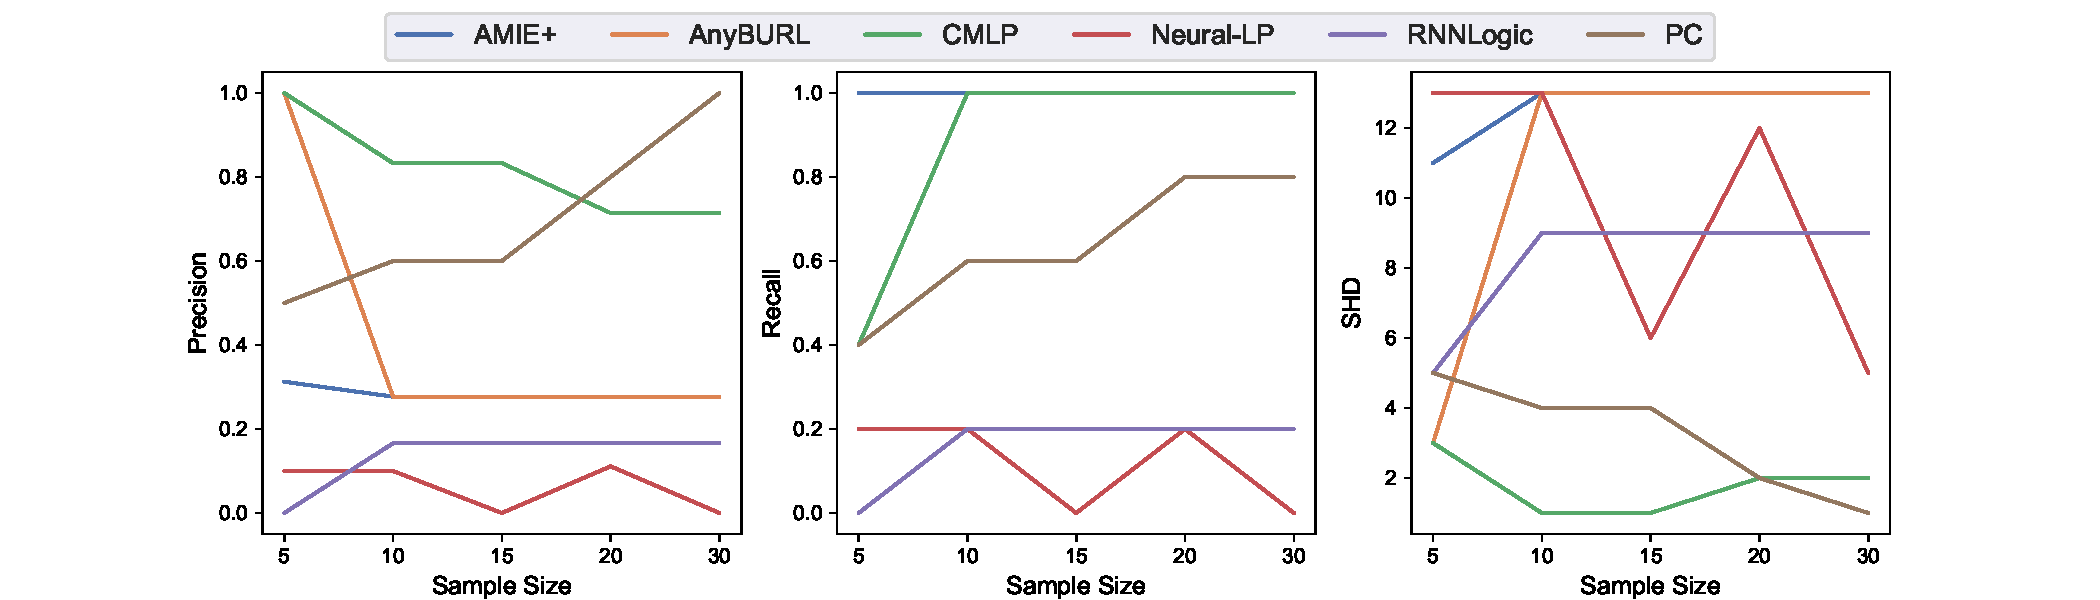
\includegraphics[trim=3cm 0cm 3cm 0cm, width=\linewidth, height=5cm]{figures/allin.pdf}
%     \caption{Precision, recall and SHD results on simulation datasets with differnet sample size. }
%     \label{fig:sim-graph}
% \end{figure*}
\noindent
\textbf{Quality of causal rules from simulations.}
The ground-truth causal graph of KGSs shown in Fig~\ref{fig:simulation}, and
Table~\ref{tab:simulation_rule_quality} shows the accuracy of estimated rules of different methods.
In particular, \dname~ accurately discovers two causal rules in Fig~\ref{fig:simulation} without any redundant rules.
In contrast, correlation-based methods report some non-causal rules.


\begin{table}[t]
\caption{Experimental results on simulation data with $p_{X_1}=0.5$, based on the metrics (precision, recall and SHD), which are commonly used to evaluate the estimated causal graph.}
%\vspace{5pt}
\label{tab:simulation_rule_quality}
\centering
\scalebox{1.2}{
\begin{tabular}{c|c|c|c}
\hline
\textbf{Method} & \textbf{Precision} $\uparrow$ & \textbf{Recall} $\uparrow$ & \textbf{SHD} $\downarrow$ \\
\hline
Neural-LP & 0 & 0& 10 \\
AMIE+ & 0.22 & \textbf{1.0}& 7 \\
RNNLogic & 0.22 & \textbf{1.0}& 7 \\
AnyBURL & 0.25 & \textbf{1.0}& 6 \\
\dname & \textbf{1.0} & \textbf{1.0} & \textbf{0} \\
\hline
\end{tabular}}
\vspace{-4pt}
\end{table}

\begin{table*}[h]
\caption{All rules whose head are $R_3$ and $R_5$, obtained by each algorithm learned on simulated dataset. The strikethroughs indicate the wrong results (there is no entities satisfying the rule).
The rules consistent with the generation process are in bold.
The orange text denotes the weight of each rule with the form max-normalization(original weight)}.

\label{tab:simulation_rule}
\centering
{\tiny
\scalebox{0.75}{
\begin{tabu}{c|l|l|l}
\tabucline[1pt]{-}
\textbf{Method} & \textbf{Rules of $R_3$ with $\mathbf{p_{X_1}=0.5}$} & \textbf{Rules of $R_3$ with $\mathbf{p_{X_1}=0.9}$} & \textbf{Rules of $R_5$}\\
\tabucline[1pt]{-}

\multirow{3}{*}{AMIE+} & \textcolor{orange}{1.00 (0.908)}   $\mathbf{R_3(C_1,C_3) \gets R_1(C_1,C_2), R_2(C_2,C_3)}$  & \textcolor{orange}{1.00 (0.900)}   $\mathbf{R_3(C_1,C_3) \gets R_1(C_1,C_2), R_2(C_2,C_3)}$ & \textcolor{orange}{1.00 (0.898)}   $R_5(C_1,C_3) \gets R_1(C_1,C_2), R_2(C_2,C_3)$\\

& \textcolor{orange}{0.91 (0.829)}   $R_3(C_1,C_3) \gets R_4(C_1,C_3)$ & \textcolor{orange}{0.99 (0.890)}   $R_3(C_1,C_3) \gets R_4(C_1,C_3)$ & \textcolor{orange}{0.99 (0.895)}   $R_5(C_1,C_3) \gets R_3(C_1,C_3)$ \\
&  \textcolor{orange}{0.55 (0.500)}   $R_3(C_1,C_3) \gets R_5(C_1,C_3)$  & \textcolor{orange}{0.91 (0.820)}   $R_3(C_1,C_3) \gets R_5(C_1,C_3)$ & \textcolor{orange}{0.99 (0.894)}   $R_5(C_1,C_3) \gets R_4(C_1,C_3)$\\
\hline
\multirow{3}{*}{AnyBURL}& \textcolor{orange}{1.00 (0.896)} $\mathbf{R_3(C_1,C_3) \gets R_1(C_1,C_2), R_2(C_2,C_3)}$ & \textcolor{orange}{1.00 (0.898)} $R_3(C_1,C_3) \gets R_4(C_1,C_3)$ & \textcolor{orange}{1.00 (0.907)} $R_5(C_1,C_3) \gets R_1(C_1,C_2), R_2(C_2,C_3)$\\
& \textcolor{orange}{0.92 (0.823)} $R_3(C_1,C_3) \gets R_4(C_1,C_3)$ &  \textcolor{orange}{0.99 (0.893)} $\mathbf{R_3(C_1,C_3) \gets R_1(C_1,C_2), R_2(C_2,C_3)}$ & \textcolor{orange}{0.99 (0.902)} $R_5(C_1,C_3) \gets R_3(C_1,C_3)$\\
& \textcolor{orange}{0.56 (0.501)} $R_3(C_1,C_3) \gets R_5(C_1,C_3)$ & \textcolor{orange}{0.91 (0.821)} $R_3(C_1,C_3) \gets R_5(C_1,C_3)$ & \textcolor{orange}{0.99 (0.897)} $R_5(C_1,C_3) \gets R_4(C_1,C_3)$ \\
\hline

\multirow{7}{*}{Neural-LP} & \textcolor{orange}{1.00 (0.318)}  \sout{$R_3(C_1,C_3) \gets R_4(C_1,C_2), R_4(C_2,C_3)$} & \textcolor{orange}{1.00 (0.757)}  \sout{$R_3(C_1,C_3) \gets R_1(C_1,C_2), R_1(C_2,C_3)$}  & \textcolor{orange}{1.00 (0.125)} \sout{$R_5(C_1,C_3) \gets R_4(C_1,C_2),R_3(C_2,C_3)$} \\
& \textcolor{orange}{0.99 (0.316)} \sout{$R_3(C_1,C_3) \gets R_4(C_1,C_2), R_5(C_2,C_3)$} & \textcolor{orange}{0.17 (0.128)} \sout{$R_3(C_1,C_3) \gets R_1(C_1,C_3)$} & \textcolor{orange}{0.78 (0.097)} \sout{$R_5(C_1,C_3) \gets R_3(C_1,C_2),R_3(C_2,C_3)$} \\
& \textcolor{orange}{0.31 (0.100)} \sout{$R_3(C_1,C_3) \gets R_5(C_1,C_2), R_4(C_2,C_3)$} & \textcolor{orange}{0.04 (0.056)} \sout{$R_3(C_1,C_3) \gets R_5(C_2,C_3), R_1(C_1,C_2)$} &\\
& \textcolor{orange}{0.31 (0.099)} \sout{$R_3(C_1,C_3) \gets R_5(C_1,C_2), R_5(C_2,C_3)$} & \textcolor{orange}{0.05 (0.035)} \sout{$R_3(C_1,C_3) \gets R_4(C_2,C_1), R_1(C_3,C_2)$} &\\
& \textcolor{orange}{0.23 (0.073)} $R_3(C_1,C_3) \gets R_4(C_1,C_3)$ & \textcolor{orange}{0.03 (0.025)} $\mathbf{R_3(C_1,C_3) \gets R_1(C_1,C_2), R_2(C_2,C_3)}$\\
& \textcolor{orange}{0.09 (0.028)} \sout{$R_3(C_1,C_3) \gets R_4(C_1,C_2), R_4(C_2,C_3)$} & \\
& \textcolor{orange}{0.07 (0.023)} $R_3(C_1,C_3) \gets R_5(C_1,C_3)$ &\\
\hline

\multirow{3}{*}{RNNLogic} & \textcolor{orange}{1.00 (0.076)}   $\mathbf{R_3(C_1,C_3) \gets R_1(C_1,C_2), R_2(C_2,C_3)}$  & \textcolor{orange}{1.00 (0.071
)}   $\mathbf{R_3(C_1,C_3) \gets R_1(C_1,C_2), R_2(C_2,C_3)}$ & \textcolor{orange}{1.00 (0.220)}   $R_5(C_1,C_3) \gets R_3(C_1,C_3)$\\

& \textcolor{orange}{0.58 (0.044)}   $R_3(C_1,C_3) \gets R_4(C_1,C_3)$ & \textcolor{orange}{0.49 (0.035)}   $R_3(C_1,C_3) \gets R_4(C_1,C_3)$ & \textcolor{orange}{0.28 (0.060)}   $R_5(C_1,C_3) \gets R_4(C_1,C_3)$ \\
&  \textcolor{orange}{0.13 (0.010)}   $R_3(C_1,C_3) \gets R_5(C_1,C_3)$  & \textcolor{orange}{0.14 (0.010)}   $R_3(C_1,C_3) \gets R_5(C_1,C_3)$ & \textcolor{orange}{0.20 (0.045)}   $R_5(C_1,C_3) \gets R_1(C_1,C_2), R_2(C_2,C_3)$\\
\hline


{\dname} & \textcolor{orange}{1.00 (122.797)} $\mathbf{R_3(C_1,C_3) \gets R_1(C_1,C_2), R_2(C_2,C_3)}$ & \textcolor{orange}{1.00 (20.061)} $\mathbf{R_3(C_1,C_3) \gets R_1(C_1,C_2), R_2(C_2,C_3)}$ & -\\

\tabucline[1pt]{-}
\end{tabu}}
}
\end{table*}

\noindent
\textbf{Interpretability of causal rules}
% For rules from the simulation, we analyze all methods' results, whose heads are $R_5$ and $R_6$, and $R_9$ and the results are shown in Table~\ref{tab:simulation_rule} .
% % The rules follow the causal mechanism are in bold.
% There is only one causal rule for $R_5$, which is $R_5(C_1,C_2) \gets R_1(C_1,C_3), R_2(C_3,C_2)$.
% AMIE+, AnyBURL, and \dname~find this causal rule.
% Besides this causal rule, the results of AMIE+ and AnyBURL also include other rules, such as $R_5(C_1,C_2) \gets R_6(C_1,C_2)$ and $R_5(C_1,C_2) \gets R_9(C_1,C_3)$.
% % Especially, for AMIE+ and AnyBURL, note that the weights of $R_3(C_1,C_3) \gets R_4(C_1,C_3)$ are very close to the weights of $R_3(C_1,C_3) \gets R_1(C_1,C_2)$, $ R_2(C_2,C_3)$.
% % It means the algorithms think these two rules have the similar interpretability for the head relation $R_3$.
% % With the change of root node $X_1$'s distribution(from $p_{X_1}=0.5$ to $p_{X_1}=0.9$), AnyBURL even report the higher weight for the rule $R_3(C_1,C_3) \gets R_5(C_1,C_3)$.
% % According to the generation mechanism, the existence of $R_3$ between entities $e_i$ and $e_j$ is independent with whether there is $R_4$ and $R_5$ between $e_i$ and $e_j$.
% % AMIE+ and AnyBURL still return these association rules with high weights, because they only consider whether $R_3$ and $R_4$ co-occur frequently, but not the reason of the co-occurrence.
% The end-to-end deep-model based method(Neural-LP and RNNLogic) fail to discover any correct rules for $R_5$.
Moreover, for the simulation dataset, we analyze all methods' results, whose heads are $R_3$ and $R_5$, and the results are shown in Table~\ref{tab:simulation_rule} (We omit results of $R_4$, since $R_3$ and $R_4$ are symmetric in the causal graph).
The rules follow the causal mechanism are in bold.
There is only one causal rule for $R_3$, which is $R_3(C_1,C_3) \gets R_1(C_1,C_2), R_2(C_2,C_3)$.
AMIE+, AnyBURL, RNNLogic and \dname~find this causal rule.
Besides this causal rule, the results of AMIE+, RNNLogic and AnyBURL also include other rules, such as $R_3(C_1,C_3) \gets R_4(C_1,C_3)$ and $R_3(C_1,C_3) \gets R_5(C_1,C_3)$.
Especially, for those three methods, note that the weights of $R_3(C_1,C_3) \gets R_4(C_1,C_3)$ are very close to the weights of $R_3(C_1,C_3) \gets R_1(C_1,C_2)$, $ R_2(C_2,C_3)$.
It means the algorithms think these two rules have the similar interpretability for the head relation $R_3$.
With the change of root node $X_1$'s distribution(from $p_{X_1}=0.5$ to $p_{X_1}=0.9$), AnyBURL even report the higher weight for the rule $R_3(C_1,C_3) \gets R_5(C_1,C_3)$.
According to the generation mechanism, the existence of $R_3$ between entities $e_i$ and $e_j$ is independent with whether there is $R_4$ and $R_5$ between $e_i$ and $e_j$.
AMIE+, AnyBURL and RNNLogic still return these association rules with high weights, because they only consider whether $R_3$ and $R_4$ co-occur frequently, but not the reason of the co-occurrence.
The end-to-end completion-oriented method, Neural-LP, also return some wrong results, such as the top 1 rule $R_3(C_1,C_3) \gets R_4(C_1,C_2), R_4(C_2,C_3)$, which can not be satisfied by any entities in KG.
The results in~\cite{sadeghian2019drum} show the same phenomenon.
The intermediate results of the completion-oriented method is incomprehensible sometimes.


Furthermore, We sort the rules generated by each algorithm based on their assigned weights and show the five top rules from Douban and Hetionet in Tab.~\ref{tab:rules_recom_result} and Tab.~\ref{tab:rule_hetionet}, respectively.
The results in Tab.~\ref{tab:rules_recom_result} suggests that the ratings for the target movie are highly related to other movies which share the same staff, such as writer, actors, director, etc.
According to the rating results, \dname~ finds a strong causal relationship between the rating of the movie and its editor than other pairs.
The top rules generated by AMIE+ and AnyBURL focus on other shared staffs, but the shared staff has different roles in the target movie and the movie in path.
Those rules of AMIE+ and AnyBURL are hard to be satisfied for most queries.
% By contrast, our mined rules suggest the ratings are determined by the subjective opinions of the users, while the mined rules from other algorithms, including AnyBURL, present the ratings are depended on others related events.
It is worth noting that RNNlogic report the `fan' rules  will impact the users' rating, but \dname~ excludes this kind of rules.
Our results suggest the working ability of the movie's stuff ({\it e.g.} actor or writer) should be the root cause of the users' rate, instead of the followers of the stuff.
From the rules from Hetionet, we can see
% Similar to the results on simulation dataset,
the learned rules are broadly divided into two classes, those in which the target drug and disease are connected by therapeutic information about the similar disease and drug, and those in which the target drug and disease are connected by commonly associated genes.
Further, we find that the rules mined by AnyBURL also contain rules for reasoning through shared side effects.



% Logically incorrect rules are highlighted by italic-red. This experiment shows two of the three top ranked rules generated by Neural LP are incorrect (for both head predicates wif e and son
\begin{table*}[t]
\centering
\caption{Top 5 Rules to infer HighRate(User, Movie) given by the methods. The strikethroughs indicate the wrong results (there is no entities satisfying the rule).
}
\label{tab:rules_recom_result}
\vspace{-1pt}
{\tiny
\begin{tabular}{c|l}
\hline
\textbf{Method} & \multicolumn{1}{c}{\textbf{ Top rules to infer HighRate(User, Movie)}} \\
\hline

\multirow{5}{*}{AMIE+} &
\textcolor{orange}{1.00 (0.565)} HighRate(User,Movie) $\gets$ HighRate(User,Movie1), Writer(Person,Movie1),Director(Person,Movie)\\
& \textcolor{orange}{0.98 (0.556)} HighRate(User,Movie) $\gets$ HighRate(User,Movie1), Director(Person,Movie1), Writer(Person,Movie)\\
& \textcolor{orange}{0.87 (0.489)} HighRate(User,Movie) $\gets$ HighRate(User,Movie1), Writer(Person,Movie1), Actress(Person,Movie)\\
& \textcolor{orange}{0.74 (0.417)} HighRate(User,Movie) $\gets$ HighRate(User,Movie1), Director(Person,Movie1), Actor(Person,Movie)\\
& \textcolor{orange}{0.72 (0.405)} HighRate(User,Movie) $\gets$ HighRate(User,Movie1), Actress(Person,Movie1), Writer(Person,Movie)\\
\hline

\multirow{5}{*}{AnyBURL} &
\textcolor{orange}{1.00 (0.400)} HighRate(User,Movie) $\gets$ HighRate(User,Movie1), Composer(Person,Movie1), Actor(Person,Movie)\\
& \textcolor{orange}{0.99(0.397)} HighRate(User,Movie) $\gets$ HighRate(User,Movie1), Producer(Person,Movie1), Director(Person,Movie)\\
& \textcolor{orange}{0.97 (0.386)} HighRate(User,Movie) $\gets$ HighRate(User,Movie1), Director(Person,Movie1), Actress(Person,Movie)\\
& \textcolor{orange}{0.89 (0.355)} HighRate(User,Movie) $\gets$ HighRate(User,Movie1), Writer(Person,Movie1), Actress(Person,Movie)\\
& \textcolor{orange}{0.85 (0.340)} HighRate(User,Movie) $\gets$ HighRate(User,Movie1), Editor(Person,Movie1), Editor(Person,Movie)\\
\hline



\multirow{2}{*}{Neural-LP}
& \textcolor{orange}{1.00 (0.120)} HighRate(User,Movie) $\gets$ HighRate(User,Movie1), HighRate(User1,Movie1), HighRate(User1,Movie)\\
& \textcolor{orange}{0.28 (0.034)} HighRate(User,Movie) $\gets$ HighRate(User,Movie1), MovieType(Movie1,Type), MovieType(Movie,Type)\\
\hline


\multirow{5}{*}{RNNLogic} &
\textcolor{orange}{1.00 (0.011)} HighRate(User,Movie) $\gets$ Fan(User,Person),Editor(Person,Movie)\\
&\textcolor{orange}{0.45 (0.005)} HighRate(User,Movie) $\gets$ Fan(User,Person),Actor(Person,Movie)\\
&\textcolor{orange}{0.36 (0.004)} HighRate(User,Movie) $\gets$ Fan(User,Person),Director(Person,Movie)\\
&\textcolor{orange}{0.36 (0.004)} HighRate(User,Movie) $\gets$ Fan(User,Person),Writer(Person,Movie)\\
&\textcolor{orange}{0.36 (0.004)} HighRate(User,Movie) $\gets$ Fan(User,Person),Composer(Person,Movie)\\
\hline

\multirow{5}{*}{\dname} &
\textcolor{orange}{1.00 (0.034)} HighRate(User,Movie) $\gets$ HighRate(User,Movie1), Editor(Person,Movie1), Editor(Person,Movie)\\

& \textcolor{orange}{0.12 (0.004)} HighRate(User,Movie1) $\gets$ HighRate(User,Movie1),Cinematographer(Person,Movie),Cinematographer(Person,Movie)
\\
& \textcolor{orange}{0.06 (0.002)} HighRate(User,Movie1) $\gets$ HighRate(User,Movie1),Writer(Person,Movie),Writer(Person,Movie)\\
& \textcolor{orange}{0.06 (0.002)} HighRate(User,Movie1) $\gets$ HighRate(User,Movie1),Actress(Person,Movie),Actress(Person,Movie)\\
& \textcolor{orange}{0.03 (0.001)} HighRate(User,Movie1) $\gets$ HighRate(User,Movie1),Director(Person,Movie),Actor(Person,Movie)\\
\hline
\end{tabular}
}
\end{table*}


\begin{table*}
\centering
\caption{Top 5 Rules to infer Treats(Compound, Disease) given by the methods. For brevity, we use `C' and `D' for compound and disease, respectively.}
\label{tab:rule_hetionet}
{\tiny
\begin{tabular}{c|l}
    \hline
    \textbf{Method} & \multicolumn{1}{c}{\textbf{ Top rules to infer Treats(Compound, Disease)}} \\ \hline
    \multirow{5}{*}{AMIE+} &
\textcolor{orange}{1.00 (0.393)}
Treats(C, D) $\gets$ Resembles(C,C1), Treats(C1, D)
    \\
& \textcolor{orange}{0.82 (0.322)}
Treats(C, D) $\gets$ Resembles(C1,C),Treats(C1, D)
\\
& \textcolor{orange}{0.42 (0.167)} Treats(C, D) $\gets$ Downregulates(C,Gene1), Associates(D,Gene1)
\\
& \textcolor{orange}{0.38 (0.151)} Treats(C, D) $\gets$ Downregulates(C,Gene1), Upregulates(D,Gene1)
 \\
& \textcolor{orange}{0.37 (0.144)} Treats(C, D) $\gets$ Binds(C,Gene1), Upregulates(D,Gene1)
\\


\hline
\multirow{5}{*}{AnyBURL} & \textcolor{orange}{1.00 (0.319)}
Treats(C, D) $\gets$ Includes(PharmacologicClass1,C),Includes(PharmacologicClass1,C1),Treats(C1, D)
 \\
& \textcolor{orange}{0.60 (0.192)}
Treats(C, D) $\gets$ Resembles(C1,C),Treats(C1, D)
 \\
& \textcolor{orange}{0.52 (0.166)}
Treats(C, D) $\gets$ Resembles(C1,C),Resembles(C1,C2),Treats(C2, D)
 \\
& \textcolor{orange}{0.31 (0.098)}
Treats(C, D) $\gets$ Resembles(C1,C),Resembles(C2,C1),Treats(C2, D)
 \\
& \textcolor{orange}{0.24 (0.077)}
Treats(C, D) $\gets$ Treats(C, D1), Resembles(D1,D)
 \\ \hline


\multirow{1}{*}{Neural-LP} &
\textcolor{orange}{1.00 (0.659)}
Treats(C, D) $\gets$ Treats(C, D1), Treats(C1, D1),Treats(C1, D)
\\ \hline



\multirow{2}{*}{RNNLogic} &
\textcolor{orange}{1.00 (0.00007)}
Treats(C, D) $\gets$ Resembles(C, C1),Treats(C1, D)
 \\
& \textcolor{orange}{1.00 (0.00007)}

Treats(C, D) $\gets$ Resembles(C, C1),
Resembles(C1, C2),Treats(C2, D)
\\ \hline


\multirow{5}{*}{\dname} &
\textcolor{orange}{1.00 (269.00))}
Treats(C, D) $\gets$ Treats(C, D1),Resembles(D1, D2),Resembles(D, D2)
 \\
    & \textcolor{orange}{0.85 (229.32))}
Treats(C, D) $\gets$ Includes(PharmacologicClass1, C),Includes(PharmacologicClass1, C1),Treats(C1, D)

\\
    & \textcolor{orange}{0.83 (224.37))}
Treats(C, D) $\gets$
Treats(C, D1),Resembles(D2, D1),Resembles(D2, D)
\\
    & \textcolor{orange}{0.58 (155.18))}
Treats(C, D) $\gets$ Treats(C, D1),Treats(C1, D1),Treats(C1, D)


\\
    & \textcolor{orange}{0.10 (26.52))}
 Treats(C, D) $\gets$
 Treats(C, D1),
 Resembles(D2,D1),
 Resembles(D,D1)

    \\ \hline

\end{tabular}
}
\end{table*}


% \begin{table*}
% \caption{Top Rules to infer $User\stackrel{Rate}{\longrightarrow}Movie$ given by the methods.}
% \label{tab:rule_douban}
% \begin{tabular}{c|l}
%     \hline
%     \textbf{Method} & \multicolumn{1}{c}{\textbf{ Top rules to infer $User\stackrel{Rate}{\longrightarrow}Movie$}} \\ \hline
%     \multirow{3}{*}{AMIE+} &
%     1. $User\stackrel{Fan}{\longrightarrow}Person\stackrel{Director}{\longrightarrow}Movie$ \\
%     & 2. $User\stackrel{Fan}{\longrightarrow}Person\stackrel{Writer}{\longrightarrow}Movie$ \\
%     & 3. $User\stackrel{Rate}{\longrightarrow}Movie1\stackrel{Director}{\longleftarrow}Person\stackrel{Director}{\longrightarrow}Movie$ \\ \hline
%     \multirow{3}{*}{AnyBURL} &  1. $User\stackrel{Rate}{\longrightarrow}Movie1\stackrel{Wish}{\longleftarrow}User1\stackrel{Rate}{\longrightarrow}Movie$ \\
%     & 2. $User\stackrel{Rate}{\longrightarrow}Movie1\stackrel{Director}{\longleftarrow}Person\stackrel{Actor}{\longrightarrow}Movie$ \\
%     & 3. $User\stackrel{Rate}{\longrightarrow}Movie1\stackrel{Producer}{\longleftarrow}Person\stackrel{Actor}{\longrightarrow}Movie$ \\ \hline
%     \multirow{3}{*}{Neural-LP} & 1. $User\stackrel{Rate}{\longrightarrow}Movie1\stackrel{Rate}{\longleftarrow}User1\stackrel{Rate}{\longrightarrow}Movie$ \\
%     & 2. $User\stackrel{Rate}{\longrightarrow}Movie1\stackrel{titleType}{\longleftarrow}MovieType\stackrel{titleType}{\longrightarrow}Movie$ \\
%     & 3. $User\stackrel{Wish}{\longrightarrow}Movie1\stackrel{archivesound}{\longleftarrow}Person\stackrel{archivesound}{\longrightarrow}Movie$ \\ \hline
%     \multirow{3}{*}{RNNLogic} & 1. $User\stackrel{Fan}{\longrightarrow}Person\stackrel{Actor}{\longrightarrow}Movie$ \\
%     & 2. $User\stackrel{Fan}{\longrightarrow}Person\stackrel{Director}{\longrightarrow}Movie$ \\
%     & 3. $User\stackrel{Fan}{\longrightarrow}Person\stackrel{Writer}{\longrightarrow}Movie$ \\ \hline
%     \multirow{3}{*}{\dname} & 1. $User\stackrel{Rate}{\longrightarrow}Movie1\stackrel{Writer}{\longleftarrow}Person\stackrel{Writer}{\longrightarrow}Movie$ \\
%     & 2. $User\stackrel{Rate}{\longrightarrow}Movie1\stackrel{Actress}{\longleftarrow}Person\stackrel{Actress}{\longrightarrow}Movie$ \\
%     & 3.$User\stackrel{Rate}{\longrightarrow}Movie1\stackrel{Director}{\longleftarrow}Person\stackrel{Actor}{\longrightarrow}Movie$ \\ \hline
% \end{tabular}
% \end{table*}

% \begin{table*}[t]
% \centering
% \caption{Top 3 Rules of HighRate given by the methods.The strikethroughs indicate the wrong results (there is no entities satisfying the rule).
% The orange text denotes the weight of each rule with the form max-normalization(original weight)}
% \label{tab:rules_recom_result}
% \vspace{-1pt}
% \begin{tabular}{c|l}
% \hline
% \textbf{Method} & \multicolumn{1}{c}{\textbf{Rules of HighRate}} \\
% \hline
% \multirow{3}{*}{Neural-LP} &
% \textcolor{orange}{1.00 (0.636)} \sout{HighRate(User,Movie) $\gets$ Saw(User1,Movie), Saw(User2,User1)}\\
%  &    \textcolor{orange}{0.50 (0.320)} \sout{HighRate(User,Movie) $\gets$ Saw(User1,Movie), Saw(User2,User1),Saw(User,User2)} \\
%   &  \textcolor{orange}{0.02(0.011)}  HighRate(User,Movie) $\gets$ Saw(User, Movie)\\
% \hline
% \multirow{3}{*}{AMIE+} &
% \textcolor{orange}{1.00 (0.662)} HighRate(User,Movie) $\gets$ Fan(User, Person), Director(Person,Movie) \\
% & \textcolor{orange}{0.99 (0.658)} HighRate(User,Movie) $\gets$ Fan(User, Person), Writer(Person,Movie) \\
% & \textcolor{orange}{0.85 (0.565)} HighRate(User,Movie) $\gets$ HighRate(User,Movie1), Writer(Person,Movie1),Director(Person,Movie)\\
% \hline
% \multirow{5}{*}{AnyBURL} &
% \textcolor{orange}{1.00 (0.286)} HighRate(User,Movie) $\gets$ HighRate(User,Movie1), Wish(User1,Movie1),HighRate(User1,Movie) \\
% & \textcolor{orange}{0.97 (0.276)} HighRate(User,Movie) $\gets$ HighRate(User,Movie1), Director(Person,Movie1),Actor(Person,Movie)
% \\
% & \textcolor{orange}{0.97 (0.276)} HighRate(User,Movie) $\gets$ HighRate(User,Movie1), Producer(Person,Movie1),Actor(Person,Movie)\\
% & $\dots$ \\
% & \textcolor{orange}{0.983 (0.236)} HighRate(User,Movie) $\gets$ Fan(User,Person), Director(Person,Movie) \\
% \hline
% \multirow{3}{*}{RNNLogic} &
% \textcolor{orange}{1.00 (0.0048)} HighRate(User,Movie) $\gets$ Fan(User,Person), Actor(Person,Movie) \\
% & \textcolor{orange}{0.875 (0.0042)} HighRate(User,Movie) $\gets$ Fan(User,Person), Director(Person,Movie) \\
% & \textcolor{orange}{0.85 (0.0041)} HighRate(User,Movie) $\gets$ Fan(User,Person), Writer(Person,Movie) \\

% \hline
% \multirow{3}{*}{\dname} &
% \textcolor{orange}{1.00 (0.035)} HighRate(User,Movie) $\gets$ HighRate(User,Movie1),Writer(Person,Movie1),Writer(Person,Movie) \\
% & \textcolor{orange}{0.06 (0.002)} HighRate(User,Movie1) $\gets$ HighRate(User,Movie1),Actress(Person,Movie),Actress(Person,Movie)
% \\
% & \textcolor{orange}{0.06 (0.002)} HighRate(User,Movie1) $\gets$ HighRate(User,Movie1),Director(Person,Movie),Actor(Person,Movie)\\
% \hline
% \end{tabular}
% \end{table*}

% We conducted an experimental study in which we investigated the performance of the learned causal rules in two aspects: the explainability to the KG and the usefulness for downstream task, such as link prediction.
% Our main goal is to provide insight into
% \begin{itemize}
%     \item the explainability of the learned causal rules to the KG.
%     \item the effectiveness of the learned causal rules or downstream task, such as link prediction.
%     \item the empirical conclusions for the hyper-parameters and alternative algorithms in our framework.
% \end{itemize}
% Furthermore, we briefly summarize the experiment designs to achieve the above-mentioned the goal under the available resources.

% Goal 1 	$\Rightarrow$ We use the simulation KG to quantitatively evaluate the learned causal rules from KG, since the causal relationships are inaccessible for real dataset\footnote{This is the most commonly used way for the evaluation of the causal discovery methods in both relational and propositional data\cite{zheng2018dags, lee2016learning}}.
% Meanwhile, the case study for real data will be introduced to qualitatively discuss the quality of mined rules.

% Goal 2 	$\Rightarrow$ 

\section{Related Work}
\label{section:related}
%\clearpage
\section{Related Work}\label{sec:related}

\noindent{\bf Parallel graph algorithms.}
There are numerous efforts that aim to parallelize generic search schemes on graphs (e.g., BFS~\cite{shun2013ligra}, DFS~\cite{naumov2017parallel}, random walk~\cite{talati2021deep}, beam search~\cite{meister2020best}, and bucketing~\cite{sridhar2019delta,zhang2020optimizing}). However, many of these algorithms were designed without considering having a vector associated with each vertex and a target of achieving high recall under a stringent latency constraint. In contrast, we analyze the search efficiency challenges of ANN and propose optimizations to handle them to allow vector-based similarity search to scale on modern multi-core architectures. Among different algorithms, the most related work to ours is perhaps $\Delta$-stepping~\cite{zhang2020optimizing}, which stages the expansion of nodes in order to avoid redundant expansions. We have applied $\Delta$-stepping to vector search and will provide a more detailed discussion in Section~\ref{subsec:delta-step} and comparison in Section~\ref{sec:eval}.

\noindent{\bf Parallel graph frameworks.}
There has been many graph engines and frameworks developed in the past decade.
Some of them are shared-memory, focusing on processing in-memory datasets within a computation node~\cite{uta2018exploring}, e.g., Galois~\cite{nguyen2013lightweight}, Ligra~\cite{shun2013ligra}, Polymer~\cite{zhang2015numa}, GraphGrind~\cite{sun2017graphgrind}, GraphIt~\cite{zhang2020optimizing}, Graptor~\cite{vandierendonck2020graptor}, and GraphBLAS~\cite{aznaveh2020parallel}.
Some are distributed systems~\cite{rivas2018mpi}, e.g., Pregel \cite{malewicz2010pregel}, GraphLab~\cite{low2014graphlab},  PowerGraph~\cite{joseph2012powergraph}, and Gluon~\cite{dathathri2019gluon}.
Some efforts focus on out-of-core designs (e.g., GraphChi~\cite{aapo2012graphchi} and X-Stream~\cite{roy2013x}) and process large graphs with disk support.
Many graph frameworks are also on GPUs~\cite{DBLP:conf/ppopp/MengLTS19}, such as CuSha~\cite{khorasani2014cusha}, Gunrock~\cite{wang2016gunrock}, GraphReduce~\cite{sengupta2015graphreduce}, Graphie~\cite{han2017graphie}, Multigraph~\cite{hong2017multigraph},  GraphBLAST~\cite{yang2019graphblast}, and Ascetic~\cite{tang2021ascetic}.
These graph systems are either based on a vertex-centric model~\cite{malewicz2010pregel,zhang2018simple} or its variants (e.g., edge-centric~\cite{roy2013x}).
Many of these parallel graph frameworks are designed primarily for generic parallel graph analytics instead of vector-based similarity search. Enabling ANN search in these frameworks, which have matured compilers and optimization technologies, is possible but requires addressing non-trivial portability challenges. For example, the input graphs of existing ANN search can have varying structures, such as hierarchical~\cite{hnsw}, heterogeneous~\cite{diskann,hm-ann}, etc. The search engine also performs additional optimizations such as transaction support~\cite{milvus}, vector reordering, prefetching, and specialized optimizations against different data types, e.g., FP32/INT8. Therefore, porting those changes, to existing frameworks, beyond the search algorithm itself, requires changes across the entire system stack.

\noindent{\bf Heterogeneous memory.}
Heterogeneous memory (HM) is emerging. It combines multiple memory components to construct main memory. HM is typically composed of a high-capacity memory technology such as non-volatile memory (but high memory access latency) and a high-performance memory technology (with limited memory capacity) such as DRAM. 
To make HM performance close to that of DRAM-only, previous work focuses on hardware-~\cite{asplos15:agarwal,hetero_mem_arch,qureshi_micro09, ibm_isca09,gpu_pcm_pact13} and software-based~\cite{eurosys16:dulloor,asplos16:lin,wen:ICS18,sc18:wu,unimem:sc17,luo:NGS,cluster20:ren} solutions to manage data placement on HM. Optane PMM and DRAM are commonly used to build HM. With PMM, the memory capacity on a single machine can achieve 6TB~\cite{optane:ucsd}. However, the latency and bandwidth of PMM is only 1/3 and 1/6 of DRAM. There are two operating modes for PMM, \textit{Memory Mode} and \textit{App-direct Mode}. 
In Memory Mode, DRAM works as a hardware-managed cache to PMM. Running the application in this mode does not require application modifications. App-direct Mode allows the programmer to explicitly control memory accesses to PMM and DRAM. \name works in App-direct Mode and outperforms Memory Mode in billion-scale dataset search (Section~\ref{sec:eval}). 

\section{Conclusion and Future work}
\label{section:conclusion}
\vspace{-.5cm}
\section{Conclusion}
\label{sec:conclusion}

Online job platforms are becoming increasingly popular.
They provide an alternative job arrangement that has the potential to dramatically affect the Future of Work. 
An increasing proportion of human workforce will be employed in such platforms.
Hence, it is very important to study the problem of platform design.
In this paper, we have a preliminary attempt at investigating this problem.
We provide a taxonomy of platforms and what are the major missing functionalities for both workers and requesters. 
We also advocate the need for interoperability between platforms.
This allows workers and requesters to move their data between platforms without getting locked into a single platform. 
There are a number of interesting research and policy challenges in achieving the vision of platform interoperability.



%\bibliographystyle{plain}
%\bibliography{submissions/causal-meta-knowledge/sample}

\begin{thebibliography}{10}

\bibitem{10.1214/ss/1177009870}
John Aldrich.
\newblock {Correlations Genuine and Spurious in Pearson and Yule}.
\newblock {\em Statistical Science}, 10(4):364 -- 376, 1995.

\bibitem{balazevic2019tucker}
Ivana Bala\v{z}evi\'c, Carl Allen, and Timothy~M Hospedales.
\newblock Tucker: Tensor factorization for knowledge graph completion.
\newblock In {\em Empirical Methods in Natural Language Processing}, 2019.

\bibitem{bordes2013translating}
Antoine Bordes, Nicolas Usunier, Alberto Garcia-Duran, Jason Weston, and Oksana
  Yakhnenko.
\newblock Translating embeddings for modeling multi-relational data.
\newblock {\em Advances in neural information processing systems}, 26, 2013.

\bibitem{chen2022fuzzy}
Xuelu Chen, Ziniu Hu, and Yizhou Sun.
\newblock Fuzzy logic based logical query answering on knowledge graphs.
\newblock In {\em Proceedings of the AAAI Conference on Artificial
  Intelligence}, volume~36, pages 3939--3948, 2022.

\bibitem{cui2011based}
Xiao Cui and Hao Shi.
\newblock A*-based pathfinding in modern computer games.
\newblock {\em International Journal of Computer Science and Network Security},
  2011.

\bibitem{evans2011metaknowledge}
James~A Evans and Jacob~G Foster.
\newblock Metaknowledge.
\newblock {\em Science}, 2011.

\bibitem{fortunato2018science}
Santo Fortunato, Carl~T Bergstrom, Katy B{\"o}rner, James~A Evans, Dirk
  Helbing, Sta{\v{s}}a Milojevi{\'c}, Alexander~M Petersen, Filippo Radicchi,
  Roberta Sinatra, Brian Uzzi, et~al.
\newblock Science of science.
\newblock {\em Science}, 2018.

\bibitem{galarraga2015fast}
Luis Gal{\'a}rraga, Christina Teflioudi, Katja Hose, and Fabian~M Suchanek.
\newblock Fast rule mining in ontological knowledge bases with amie.
\newblock {\em The VLDB Journal}, 24(6):707--730, 2015.

\bibitem{galarraga2013amie}
Luis~Antonio Gal{\'a}rraga, Christina Teflioudi, Katja Hose, and Fabian
  Suchanek.
\newblock Amie: association rule mining under incomplete evidence in
  ontological knowledge bases.
\newblock In {\em Proceedings of the 22nd international conference on World
  Wide Web}, pages 413--422, 2013.

\bibitem{galarraga_amie_2013}
Luis~Antonio Galárraga, Christina Teflioudi, Katja Hose, and Fabian Suchanek.
\newblock {AMIE}: association rule mining under incomplete evidence in
  ontological knowledge bases.
\newblock In {\em Proceedings of the 22nd international conference on World
  Wide Web - {WWW} '13}, pages 413--422. {ACM} Press.

\bibitem{gerhardus2020high}
Andreas Gerhardus and Jakob Runge.
\newblock High-recall causal discovery for autocorrelated time series with
  latent confounders.
\newblock {\em Advances in Neural Information Processing Systems},
  33:12615--12625, 2020.

\bibitem{giudice2022dual}
Enrico Giudice, Jack Kuipers, and Giusi Moffa.
\newblock The dual pc algorithm for structure learning.
\newblock In {\em International Conference on Probabilistic Graphical Models},
  pages 301--312. PMLR, 2022.

\bibitem{glymour2016causal}
Madelyn Glymour, Judea Pearl, and Nicholas~P Jewell.
\newblock {\em Causal inference in statistics: A primer}.
\newblock John Wiley \& Sons, 2016.

\bibitem{heusner2018best}
Manuel Heusner, Thomas Keller, and Malte Helmert.
\newblock Best-case and worst-case behavior of greedy best-first search.
\newblock International Joint Conferences on Artificial Intelligence, 2018.

\bibitem{himmelstein2017systematic}
Daniel~Scott Himmelstein, Antoine Lizee, Christine Hessler, Leo Brueggeman,
  Sabrina~L Chen, Dexter Hadley, Ari Green, Pouya Khankhanian, and Sergio~E
  Baranzini.
\newblock Systematic integration of biomedical knowledge prioritizes drugs for
  repurposing.
\newblock {\em Elife}, 6:e26726, 2017.

\bibitem{imbens2010rubin}
Guido~W Imbens and Donald~B Rubin.
\newblock Rubin causal model.
\newblock In {\em Microeconometrics}, pages 229--241. Springer, 2010.

\bibitem{ji2021survey}
Shaoxiong Ji, Shirui Pan, Erik Cambria, Pekka Marttinen, and S~Yu Philip.
\newblock A survey on knowledge graphs: Representation, acquisition, and
  applications.
\newblock {\em IEEE Transactions on Neural Networks and Learning Systems},
  33(2):494--514, 2021.

\bibitem{lanning2014dijkstra}
Daniel~R Lanning, Gregory~K Harrell, and Jin Wang.
\newblock Dijkstra's algorithm and google maps.
\newblock In {\em Proceedings of the 2014 ACM Southeast Regional Conference},
  2014.

\bibitem{le2016fast}
Thuc~Duy Le, Tao Hoang, Jiuyong Li, Lin Liu, Huawen Liu, and Shu Hu.
\newblock A fast pc algorithm for high dimensional causal discovery with
  multi-core pcs.
\newblock {\em IEEE/ACM transactions on computational biology and
  bioinformatics}, 16(5):1483--1495, 2016.

\bibitem{lee2016learning}
Sanghack Lee and Vasant Honavar.
\newblock On learning causal models from relational data.
\newblock In {\em Thirtieth AAAI Conference on Artificial Intelligence}, 2016.

\bibitem{lee2020towards}
Sanghack Lee and Vasant Honavar.
\newblock Towards robust relational causal discovery.
\newblock In {\em Uncertainty in Artificial Intelligence}. PMLR, 2020.

\bibitem{li2021kg4vis}
Haotian Li, Yong Wang, Songheng Zhang, Yangqiu Song, and Huamin Qu.
\newblock Kg4vis: A knowledge graph-based approach for visualization
  recommendation.
\newblock {\em IEEE Transactions on Visualization and Computer Graphics},
  28(1):195--205, 2021.

\bibitem{lin2021multi}
Zizheng Lin, Haowen Ke, Ngo-Yin Wong, Jiaxin Bai, Yangqiu Song, Huan Zhao, and
  Junpeng Ye.
\newblock Multi-relational graph based heterogeneous multi-task learning in
  community question answering.
\newblock In {\em Proceedings of the 30th ACM International Conference on
  Information \& Knowledge Management}, pages 1038--1047, 2021.

\bibitem{maier2013sound}
Marc Maier, Katerina Marazopoulou, David Arbour, and David Jensen.
\newblock A sound and complete algorithm for learning causal models from
  relational data.
\newblock In {\em Uncertainty in Artificial Intelligence}, page 371. Citeseer,
  2013.

\bibitem{maier2010learning}
Marc Maier, Brian Taylor, Huseyin Oktay, and David Jensen.
\newblock Learning causal models of relational domains.
\newblock In {\em Proceedings of the AAAI Conference on Artificial
  Intelligence}, 2010.

\bibitem{marx2019testing}
Alexander Marx and Jilles Vreeken.
\newblock Testing conditional independence on discrete data using stochastic
  complexity.
\newblock In {\em The 22nd International Conference on Artificial Intelligence
  and Statistics}, 2019.

\bibitem{meilicke2019anytime}
Christian Meilicke, Melisachew~Wudage Chekol, Daniel Ruffinelli, and Heiner
  Stuckenschmidt.
\newblock Anytime bottom-up rule learning for knowledge graph completion.
\newblock In {\em IJCAI}, pages 3137--3143, 2019.

\bibitem{omran2019embedding}
Pouya~Ghiasnezhad Omran, Kewen Wang, and Zhe Wang.
\newblock An embedding-based approach to rule learning in knowledge graphs.
\newblock {\em IEEE Transactions on Knowledge and Data Engineering}, 2019.

\bibitem{pearl2010causal}
Judea Pearl.
\newblock Causal inference.
\newblock {\em Causality: Objectives and Assessment}, pages 39--58, 2010.

\bibitem{qu2020rnnlogic}
Meng Qu, Junkun Chen, Louis-Pascal Xhonneux, Yoshua Bengio, and Jian Tang.
\newblock Rnnlogic: Learning logic rules for reasoning on knowledge graphs.
\newblock In {\em International Conference on Learning Representations}, 2021.

\bibitem{ratajczak2022task}
Florin Ratajczak, Mitchell Joblin, Martin Ringsquandl, and Marcel Hildebrandt.
\newblock Task-driven knowledge graph filtering improves prioritizing drugs for
  repurposing.
\newblock {\em BMC bioinformatics}, 23(1):1--19, 2022.

\bibitem{rossi2021knowledge}
Andrea Rossi, Denilson Barbosa, Donatella Firmani, Antonio Matinata, and Paolo
  Merialdo.
\newblock Knowledge graph embedding for link prediction: A comparative
  analysis.
\newblock {\em ACM Transactions on Knowledge Discovery from Data (TKDD)},
  15(2):1--49, 2021.

\bibitem{ruffinelli2020you}
Daniel Ruffinelli, Samuel Broscheit, and Rainer Gemulla.
\newblock You can teach an old dog new tricks! on training knowledge graph
  embeddings.
\newblock 2020.

\bibitem{sadeghian2019drum}
Ali Sadeghian, Mohammadreza Armandpour, Patrick Ding, and Daisy~Zhe Wang.
\newblock Drum: End-to-end differentiable rule mining on knowledge graphs.
\newblock {\em Advances in Neural Information Processing Systems}, 32, 2019.

\bibitem{salimi2020causal}
Babak Salimi, Harsh Parikh, Moe Kayali, Lise Getoor, Sudeepa Roy, and Dan
  Suciu.
\newblock Causal relational learning.
\newblock In {\em Proceedings of the 2020 ACM SIGMOD International Conference
  on Management of Data}, 2020.

\bibitem{sondhi2019reduced}
Arjun Sondhi and Ali Shojaie.
\newblock The reduced pc-algorithm: Improved causal structure learning in large
  random networks.
\newblock {\em J. Mach. Learn. Res.}, 20(164):1--31, 2019.

\bibitem{spirtes2000causation}
Peter Spirtes, Clark~N Glymour, Richard Scheines, and David Heckerman.
\newblock {\em Causation, prediction, and search}.
\newblock MIT press, 2000.

\bibitem{tang2020investigating}
Xianfeng Tang, Huaxiu Yao, Yiwei Sun, Yiqi Wang, Jiliang Tang, Charu Aggarwal,
  Prasenjit Mitra, and Suhang Wang.
\newblock Investigating and mitigating degree-related biases in graph
  convoltuional networks.
\newblock In {\em Proceedings of the 29th ACM International Conference on
  Information \& Knowledge Management}, pages 1435--1444, 2020.

\bibitem{tiwari2021revisiting}
Sudhanshu Tiwari, Iti Bansal, and Carlos~R Rivero.
\newblock Revisiting the evaluation protocol of knowledge graph completion
  methods for link prediction.
\newblock In {\em Proceedings of the Web Conference 2021}, pages 809--820,
  2021.

\bibitem{wang2019multi}
Hongwei Wang, Fuzheng Zhang, Miao Zhao, Wenjie Li, Xing Xie, and Minyi Guo.
\newblock Multi-task feature learning for knowledge graph enhanced
  recommendation.
\newblock In {\em The World Wide Web Conference}, 2019.

\bibitem{wang2019kgat}
Xiang Wang, Xiangnan He, Yixin Cao, Meng Liu, and Tat-Seng Chua.
\newblock Kgat: Knowledge graph attention network for recommendation.
\newblock In {\em Proceedings of the 25th ACM SIGKDD International Conference
  on Knowledge Discovery \& Data Mining}, 2019.

\bibitem{wang2021benchmarking}
Zihao Wang, Hang Yin, and Yangqiu Song.
\newblock Benchmarking the combinatorial generalizability of complex query
  answering on knowledge graphs.
\newblock In {\em NeurIPS Datasets and Benchmarks Track}, 2021.

\bibitem{wu2021self}
Jiancan Wu, Xiang Wang, Fuli Feng, Xiangnan He, Liang Chen, Jianxun Lian, and
  Xing Xie.
\newblock Self-supervised graph learning for recommendation.
\newblock In {\em Proceedings of the 44th international ACM SIGIR conference on
  research and development in information retrieval}, pages 726--735, 2021.

\bibitem{yang2017differentiable}
Fan Yang, Zhilin Yang, and William~W Cohen.
\newblock Differentiable learning of logical rules for knowledge base
  reasoning.
\newblock {\em Advances in neural information processing systems}, 30, 2017.

\bibitem{zhang2020aser}
Hongming Zhang, Xin Liu, Haojie Pan, Yangqiu Song, and Cane Wing-Ki Leung.
\newblock Aser: A large-scale eventuality knowledge graph.
\newblock In {\em Proceedings of the web conference 2020}, pages 201--211,
  2020.

\bibitem{zheng2018dags}
Xun Zheng, Bryon Aragam, Pradeep Ravikumar, and Eric~P. Xing.
\newblock {DAGs with NO TEARS: Continuous Optimization for Structure Learning}.
\newblock In {\em Advances in Neural Information Processing Systems}, 2018.

\bibitem{zheng2020learning}
Xun Zheng, Chen Dan, Bryon Aragam, Pradeep Ravikumar, and Eric~P. Xing.
\newblock {Learning sparse nonparametric DAGs}.
\newblock In {\em International Conference on Artificial Intelligence and
  Statistics}, 2020.

\end{thebibliography}

\end{document}

